\documentclass[journal]{IEEEtran}
% *** MATH PACKAGES ***
\usepackage{amsmath}
% *** PDF, URL AND HYPERLINK PACKAGES ***
\usepackage{hyperref}
\hypersetup{
    %colorlinks=true,
    %linkcolor=blue,
    %filecolor=magenta,
    %urlcolor=cyan,
}
\urlstyle{same}
\hyphenation{op-tical net-works semi-conduc-tor}
\usepackage{graphicx}
\usepackage{float}
\usepackage{tabularx}

\begin{document}

\title{Autonomous Network for Coastal Hardware and Operational Reporting System}

\author{
\IEEEauthorblockN{Jay Gnanasekaran\IEEEauthorrefmark{2}}\\
\IEEEauthorblockA{\IEEEauthorrefmark{2}Johns Hopkins University, Whiting School of Engineering, Computer Science Department\\
\emph{jgnanas1@jh.edu}}
}

\markboth{EN.605.636.SP26 Autonomic Computing Project Proposal}{}
\maketitle

\begin{abstract}
In this paper, I explore the system architecture needed to provide an autonomic computing system for remotely deployed maritime devices. These devices, referred to as MARLINs (Maritime Autonomous Remote Linked Intelligence Nodes), are conceived as floating sensor platforms equipped with GPS, temperature and humidity sensing, Wi-Fi scanning capability, and low-bandwidth communication back to a command console. The autonomic manager for this system is ANCHOR, Autonomous Network for Coastal Hardware and Operational Reporting. The original design goal of the project was to place the full autonomic manager directly on each MARLIN. However, as the prototype evolved, practical constraints in current LLM tooling, execution safety, and edge-device limitations led to a hybrid realization in which local policy enforcement remains on the MARLIN while higher-order reasoning is centralized at the ANCHOR base station. This research investigates whether such a hybrid MAPE-K architecture, supported by Codex as a reasoning engine, can still reduce required human monitoring by at least 65 percent while preserving core autonomic behaviors.
\end{abstract}

\begin{IEEEkeywords}
MAPE-K, autonomic computing, edge systems, remote sensor nodes, LLM agents
\end{IEEEkeywords}

\section{Introduction}~\label{intro}
\IEEEPARstart{R}{emotely} deployed maritime devices present a unique challenge for systems management. Unlike a server in a data center or a container in a cloud environment, a floating sensor node cannot be physically reached when something goes wrong. It may be miles offshore, operating in rough weather, with only a low-bandwidth radio link back to shore. Current solutions to this problem rely heavily on human operators monitoring device telemetry and issuing corrective commands when anomalies appear. This current implementation is sufficient, but it is expensive in man-hours, introduces response latency, and creates a single point of failure whenever an operator is unavailable.

The goal of this project is to reduce that dependency by embedding autonomic behavior into a maritime sensing system. ANCHOR, or Autonomous Network for Coastal Hardware and Operational Reporting, is designed to monitor the health and mission state of its host MARLIN (Maritime Autonomous Remote Linked Intelligence Node), reason about faults and environmental changes, and take corrective action with minimal human intervention. The original vision of the project was a fully decentralized architecture in which each MARLIN hosted its own complete autonomic manager. As implementation progressed, however, that vision had to be adapted to account for the realities of current LLM tooling, execution safety, and edge-device constraints. The resulting prototype remains faithful to the MAPE-K autonomic computing model, but realizes it as a hybrid system in which local autonomy is preserved at the node while reasoning-intensive functions are centralized at the base station.

\section{Research Statement}~\label{statement}
This research investigates whether an LLM-based autonomic manager, built on the MAPE-K framework and implemented as a hybrid edge-and-base-station system, can reduce the need for human intervention in remotely deployed maritime sensor nodes by at least 65\%. In the realized prototype, MARLIN nodes perform local sensing, local mission-policy enforcement, and fail-safe mode transitions, while the ANCHOR base station performs higher-order analysis, fleet coordination, and constrained command generation through Codex.

\section{Background}~\label{background}
This research brings together several technologies to form the ANCHOR system: remote maritime sensing platforms, autonomic computing principles, lightweight edge-node control, centralized fleet coordination, and LLM-supported reasoning.

\subsection{MARLINs}
MARLINs, or Maritime Autonomous Remote Linked Intelligence Nodes, are the remote devices used in this research. Although motivated by maritime deployment, the concept could be generalized to any device placed in an inaccessible location: buried underground, deployed in mountainous terrain, or otherwise physically unreachable during normal operation. In this project, however, MARLINs are specifically imagined as floating buoy-like systems operating on the surface of the water.

The original hardware concept for a MARLIN includes a Raspberry Pi 4, a GPS module, a temperature and humidity sensor, a Wi-Fi interface for local scan activity, a LoRa radio for low-bandwidth communication, and a battery-backed enclosure suitable for deployment at sea. In the current prototype, many of these hardware elements are simulated so that the autonomic behavior of the system can be validated before a full hardware deployment is attempted. The live field test described later therefore used an Ubuntu laptop as the MARLIN host rather than a fully integrated Raspberry Pi buoy enclosure. The system described in this paper is therefore a project prototype developed for this research effort rather than a production deployment used in my workplace.

\subsection{Codex}
Codex is an agentic coding tool developed by OpenAI that operates through a command-line interface powered by a large language model~\cite{openai_codex_2025}. Unlike a traditional code assistant that responds to isolated prompts, Codex can reason over a codebase, plan multi-step tasks, run terminal commands, and iterate on its own output. It is designed to function as an autonomous software agent rather than as a pure text generator.

In this project, Codex serves as the higher-order reasoning engine behind ANCHOR. Rather than implementing only a rigid rule-based manager, ANCHOR uses Codex to interpret incoming telemetry, suggest mission-aware actions, and adapt to novel conditions. Earlier project planning considered Claude Code as the agentic tool in this role, but the realized prototype adopted Codex because its command-line workflow, repository reasoning, and tool-driven execution model fit the implementation needs of the project more directly. Within the autonomic loop, Codex functions as the analyze-and-plan mechanism for ANCHOR rather than as a separate operator convenience layer. However, Codex is not granted unrestricted shell-level authority over remote devices. Instead, it operates within a constrained command model in which all actions must conform to a predefined schema and pass policy validation before they are sent to a MARLIN node. This distinction between unrestricted execution and bounded operational autonomy became an important design outcome of the project.

\section{Related Work}~\label{related}
Several areas of prior research inform this project: unattended remote sensor networks, autonomic computing frameworks, self-healing wireless systems, and LLM-based agentic management.

\subsection{Unattended Ground Sensor Networks}
One of the closest parallels to the MARLIN system is the DARPA Unattended Ground Sensor (UGS) research program. These sensors were designed to be randomly deployed in inaccessible environments and to operate for long periods without physical maintenance. Like MARLINs, they communicated over constrained radio links and had to make decisions about power, topology, and transmission without direct human intervention.

Gilbert and Talmadge explored how these sensors could continue functioning under sub-optimal atmospheric conditions that degrade radio transmissions~\cite{gilbert1997ugs}. Their work on adaptive transmission algorithms is directly relevant to how ANCHOR handles degraded connectivity. The UGS program also demonstrated patterns of self-configuration and autonomous wake-sleep behavior that are conceptually aligned with this project.

\subsection{Self-Healing Wireless Sensor Networks}
Vlajic and Moniz examine how wireless sensor networks can continue operating when individual nodes fail or become unreachable~\cite{vlajic2007selfhealing}. Their findings on rerouting, graceful degradation, and fault isolation translate directly to the MARLIN use case, where a node going dark should not necessarily imply full mission failure. In this project, the same principle appears in MARLIN's ability to continue operating from cached mission policy even when disconnected from ANCHOR.

\subsection{The Vision of Autonomic Computing}
Kephart and Chess formalized the case for autonomic computing in response to the growing difficulty of managing complex distributed systems~\cite{kephart2003vision}. Their MAPE-K framework remains the dominant model for self-managing systems and is the architectural foundation for ANCHOR. Their central argument, that systems should manage themselves in the background with minimal human effort, directly motivates the design of a maritime node capable of passive operation and automatic adaptation.

\subsection{LLM Agents in Systems Management}
The use of large language models as reasoning engines within autonomic loops is an emerging area. Recent work has shown that LLMs can plan multi-step tasks, use external tools, and correct their own outputs in an agentic setting~\cite{yao2023react}. ANCHOR applies this directly by replacing a purely hand-coded analyze-and-plan engine with Codex, allowing the manager to reason about telemetry and mission state in natural language. At the same time, this project also exposes a practical limit of current technology: while LLM reasoning is valuable, unrestricted execution on remote edge devices is not yet a realistic or safe default for a robust autonomic prototype.

\section{Proposed Project}~\label{design}
This project proposes the design and implementation of ANCHOR, Autonomous Network for Coastal Hardware and Operational Reporting. The original concept placed the complete autonomic manager directly onboard each MARLIN. The realized prototype instead implements ANCHOR as a hybrid autonomic system composed of multiple MARLIN edge nodes and a centralized ANCHOR base station.

\subsection{System Overview}
In the prototype, each MARLIN is responsible for local sensing, mission-policy evaluation, mode switching, local state caching, and execution of a restricted set of structured commands. The ANCHOR base station receives telemetry from all MARLINs, stores fleet state and mission history, provides an operator dashboard and chat interface, and invokes Codex for higher-order reasoning and command generation.

Each MARLIN collects GPS position, battery level, temperature and humidity, and nearby Wi-Fi observations. These readings are assembled into a structured snapshot and sent to ANCHOR according to the current mission configuration. Reporting frequency is not globally fixed. Instead, it is determined by mission policy and may change depending on whether the node is operating passively, actively scanning, or conserving power. The dashboard and chat interface expose this state to an operator, but they are not themselves the autonomic control mechanism. The control logic remains in MARLIN's local policy engine and ANCHOR's reasoning-and-command path.

ANCHOR maintains a long-lived mission configuration for each MARLIN. This mission configuration includes an active geofence, passive and active reporting intervals, Wi-Fi scan policy, and permitted operational routines. MARLIN caches this mission configuration locally so that it can continue to function even if communication with ANCHOR is interrupted.

\subsection{From Intended to Realized Architecture}
The original design goal of this project was to implement ANCHOR as a fully decentralized autonomic manager running directly on each MARLIN node. In that intended architecture, every MARLIN would host its own complete MAPE-K loop, including local monitoring, analysis, planning, execution, and knowledge management. The central command console would serve primarily as a passive dashboard for human visibility and occasional override, while the MARLINs themselves would remain operationally independent.

As the prototype moved from concept to implementation, however, several practical constraints emerged. First, current large language model tooling is better suited to a connected base-station environment than to a resource-constrained edge device. While the original proposal envisioned Codex running as a local reasoning engine onboard each Raspberry Pi, the realities of edge compute limits, network dependence, and runtime tooling made that approach difficult to implement reliably in a prototype. Second, granting an LLM unrestricted shell-level control over a remote device introduced safety and validation concerns that were inconsistent with a robust systems design. In practice, a constrained command interface proved more realistic than fully open-ended agent execution.

These constraints led to an architectural adaptation. In the realized prototype, MARLIN remains responsible for local sensing, geofence-based mission evaluation, mode switching, local caching, and execution of a predefined set of structured commands. ANCHOR, running at the base station, performs fleet coordination, mission management, telemetry storage, operator interaction, and higher-order reasoning through Codex. Rather than executing arbitrary shell commands, Codex operates within a bounded action model in which all proposed actions must conform to a validated schema and mission policy before being issued to a MARLIN.

This change does not eliminate the autonomic computing objective of the project. Instead, it refines that objective into a hybrid architecture that better reflects current technological realities. The realized system still preserves autonomic behavior at the edge through local policy enforcement and fail-safe operation, while centralizing reasoning-intensive functions at the base station. As a result, the prototype serves both as an implementation of a practical autonomic maritime management system and as an evaluation of the current gap between ideal decentralized autonomy and what contemporary LLM-based systems can reliably support.

\subsection{MAPE-K Implementation}
The ANCHOR prototype follows the MAPE-K model, but distributes its phases across the MARLIN node and the ANCHOR base station.

\textbf{Monitor:} MARLIN performs the monitor function locally by collecting GPS, battery, temperature and humidity, and Wi-Fi scan data. It packages these readings into structured snapshots and emits asynchronous events such as geofence entry, low battery, target detection, or command failure.

\textbf{Analyze:} ANCHOR performs higher-order analysis at the base station. Incoming snapshots and events are stored in the fleet database and used by ANCHOR's \texttt{reasoning\_engine.py} component to determine whether Codex should be invoked. Automatic reasoning is triggered on selected events such as geofence entry, target detection, low battery, command failure, or mission configuration changes. MARLIN also performs a limited form of local analysis through its rule-based mission evaluator, but that logic is intentionally bounded to predefined geofence and battery rules rather than a full onboard LLM-driven analyze phase.

\textbf{Plan:} Codex serves as the planning engine within ANCHOR. It receives a structured context packet, represented in the implementation as a JSON-serializable dictionary containing the trigger, the current node summary, the active mission configuration, recent history, and the set of allowed actions. Codex returns a summary, a set of recommended structured commands, an optional mission configuration patch, and a confidence score. On MARLIN, limited local planning exists only in the sense that predefined responses are selected when specific local rules are met.

\textbf{Execute:} Execution is split between ANCHOR and MARLIN. ANCHOR validates proposed actions through a policy guard before issuing commands. MARLIN receives only structured commands, validates them locally, and executes them through predefined handlers. Codex therefore operates with bounded operational autonomy rather than unrestricted command-line control.

\textbf{Knowledge:} Knowledge is distributed across the system. ANCHOR maintains the fleet database, mission history, operator interactions, reasoning outputs, commands, and command results. MARLIN maintains a lightweight local cache consisting of its current mission configuration, current node state, and an outbound queue of unsent snapshots, events, and command responses.

\subsection{Communication and Offline Behavior}
If communication between a MARLIN and ANCHOR is lost, the MARLIN continues operating using its cached mission configuration. It continues evaluating geofence conditions locally, maintains its current mode, applies low-battery protections, queues snapshots and events for later upload, and resumes transmission when contact returns. In other words, events such as geofence transitions and low-power mode changes are still detected and handled on the MARLIN even while ANCHOR is disconnected. This behavior is important because it preserves edge autonomy even though higher-order reasoning has been centralized.

\subsection{Implementation Plan}
The project proceeds in three phases. In the first phase, a simulated MARLIN environment is built on a local machine to validate the MAPE-K loop, the telemetry model, and Codex integration without requiring full physical hardware. Sensor inputs are simulated and fault conditions are injected manually to test ANCHOR's responses. In the second phase, the system is deployed on a physical Raspberry Pi or equivalent Linux-based node with selected live sensors connected. In the third phase, a multi-node scenario is tested in which multiple MARLINs report to a single ANCHOR base station, validating fleet tracking, mission coordination, and multi-node reasoning behavior.

\begin{figure}[H]
\begin{center}
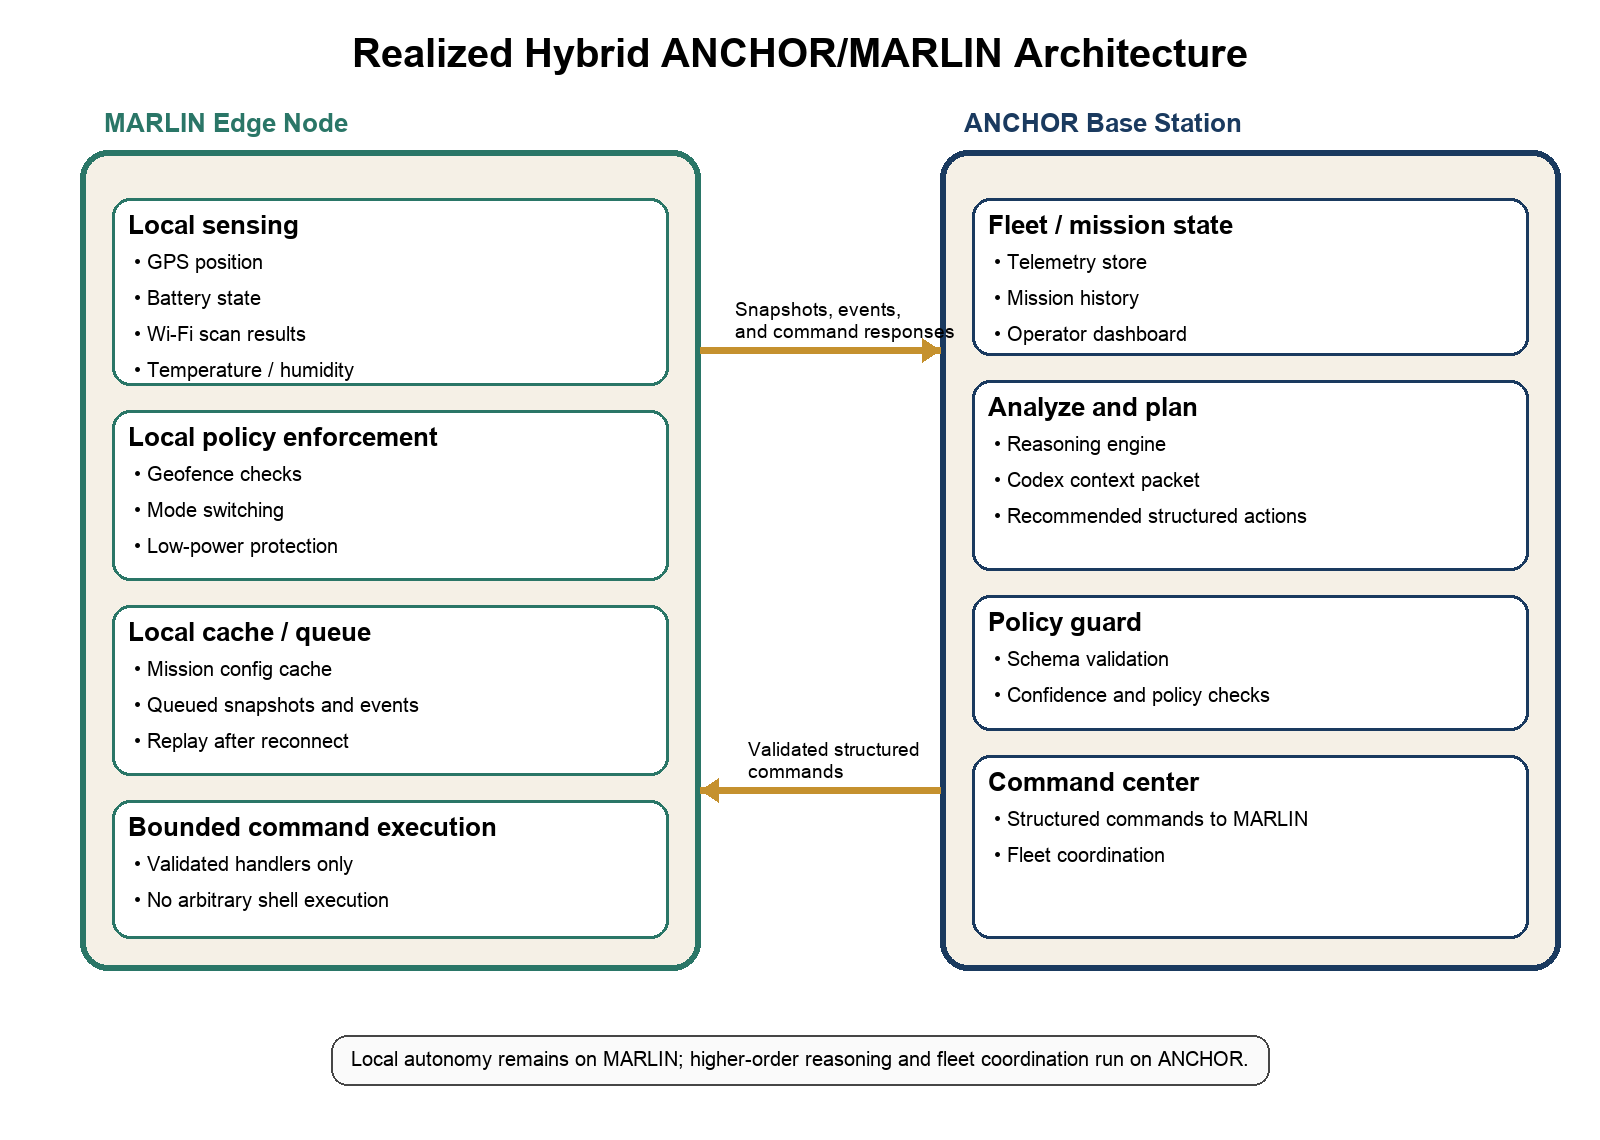
\includegraphics[width=0.48\textwidth]{images/anchor_marlin_architecture.png}
\caption{Project-specific view of the realized hybrid architecture. MARLIN performs sensing, local policy enforcement, caching, and bounded command execution, while ANCHOR performs fleet coordination, reasoning, and validated command generation.}
\label{fig:autonomic}
\end{center}
\end{figure}

\section{Software Stack}~\label{stack}
The realized ANCHOR prototype is implemented in Python and organized as a single repository containing three major components: a shared protocol layer, a MARLIN node runtime, and an ANCHOR base-station runtime. This structure reflects the hybrid architecture of the prototype, where telemetry collection and local policy enforcement occur at the edge while higher-order reasoning, fleet coordination, and operator interaction are centralized at the base station.

The software stack was designed with two practical goals in mind. First, it needed to remain simple enough to support rapid iteration in a research setting. Second, it needed to preserve enough architectural separation to reflect the intended operational roles of MARLIN and ANCHOR. As a result, the implementation uses plain Python modules, JSON-based message structures, lightweight local persistence, and a browser-based dashboard rather than a heavyweight distributed framework.

\subsection{Repository Structure}
The prototype codebase is organized into four main areas:

\begin{verbatim}
shared/
  mission_config.py
  anchor_command.py
  snapshot.py
  event.py
  command_response.py

marlin/
  gps_reader.py
  wifi_scanner.py
  temp_humidity_reader.py
  battery_reader.py
  snapshot_builder.py
  mission_evaluator.py
  command_handler.py
  wifi_task_runner.py
  uploader.py
  local_store.py
  main.py

anchor/
  api_server.py
  database.py
  fleet_manager.py
  mission_manager.py
  map_tracker.py
  command_center.py
  reasoning_engine.py
  policy_guard.py
  main.py

web/
  index.html
\end{verbatim}

This structure separates the communication schema, the edge-node runtime, the base-station runtime, and the operator-facing interface. Although implemented as a single repository, MARLIN and ANCHOR remain conceptually distinct programs that would be deployed on different machines in a realistic setting. At runtime, they communicate through structured HTTP/JSON messages defined in the shared protocol layer rather than by using the repository itself as a communication channel.

\subsection{Shared Protocol Layer}
The \texttt{shared/} directory defines the message structures exchanged between MARLIN and ANCHOR. These structures act as the protocol contract between the edge node and the base station.

\texttt{mission\_config.py} defines the long-lived mission policy distributed by ANCHOR to each MARLIN. The mission configuration includes the node identifier, a single active geofence, passive and active reporting intervals, Wi-Fi scan policy, authorized targets, approved routines, and sleep rules. This configuration is cached locally on MARLIN so that the node can continue operating even if communication with ANCHOR is interrupted.

\texttt{anchor\_command.py} defines the structured command model used by ANCHOR to instruct a MARLIN. Rather than transmitting arbitrary shell commands, ANCHOR sends validated commands such as mode changes, snapshot requests, Wi-Fi scan requests, sleep conditions, or mission configuration updates. This file also defines the set of valid command types and allowable mode values.

\texttt{snapshot.py}, \texttt{event.py}, and \texttt{command\_response.py} define the three primary classes of outbound messages sent by MARLIN. A snapshot is routine telemetry, an event is an asynchronous state change or alert, and a command response communicates whether a previously issued command was accepted, rejected, completed, or failed.

This protocol layer is important because it transforms autonomy from open-ended command execution into a constrained message-based system. That design choice supports validation, traceability, and safer experimentation with Codex-generated actions.

\subsection{MARLIN Runtime}
The \texttt{marlin/} directory implements the remote node behavior. In the realized prototype, MARLIN acts as a policy-driven edge agent rather than a full onboard autonomic manager.

\texttt{gps\_reader.py}, \texttt{temp\_humidity\_reader.py}, \texttt{battery\_reader.py}, and \texttt{wifi\_scanner.py} represent the local sensing layer. In the current prototype these may return mocked values, but they are organized so they can later be replaced by live hardware integrations. In the final prototype used for field testing, \texttt{gps\_reader.py} was adapted to consume a live NMEA stream from a mobile hotspot, \texttt{battery\_reader.py} was adapted to read the host laptop's battery percentage, and \texttt{wifi\_scanner.py} was adapted to invoke the local wireless interface through Linux command-line tools.

\texttt{snapshot\_builder.py} assembles the current node state into a structured snapshot object. This includes position, battery information, environmental readings, Wi-Fi scan metadata, and any collected Wi-Fi observations. By centralizing snapshot construction, the code ensures that all telemetry sent to ANCHOR follows a consistent format.

\texttt{mission\_evaluator.py} is one of the most important MARLIN modules. It compares the current GPS position against the active geofence defined in the mission configuration and determines whether the node should be operating in passive mode, active mode, or low-power mode. This preserves a key autonomic property locally: MARLIN can still react to its mission state even when disconnected from the base station.

\texttt{command\_handler.py} validates and acknowledges structured commands received from ANCHOR. It produces command responses indicating whether a command was accepted and later whether it completed successfully. This module is part of the local execution safety model, since MARLIN does not blindly execute raw external instructions.

\texttt{wifi\_task\_runner.py} contains predefined Wi-Fi routines such as active scanning, monitoring, and stop actions. These routines are deliberately bounded. Their existence reinforces the architectural decision that ANCHOR and Codex may select from allowed operations, but may not improvise arbitrary shell-level behavior on the remote node.

\texttt{uploader.py} is responsible for queueing outbound messages and, in a more complete implementation, would manage transmission to the ANCHOR base station. The current prototype uses a lightweight queue-oriented approach appropriate to intermittent connectivity.

\texttt{local\_store.py} implements flat-file persistence for node-local state. MARLIN stores its current mission configuration, current node state, and an outbound queue of unsent messages. This design reflects the requirement that a disconnected node must remain operational using its last known policy.

\texttt{main.py} serves as the MARLIN entry point and coordinates the local cycle of reading sensors, evaluating mission state, building snapshots, updating local state, and queueing outbound telemetry. In the field-tested version of the prototype, \texttt{main.py} was extended to run a periodic background loop so that MARLIN could continue sensing and evaluating geofence conditions autonomously without requiring a manual trigger for each telemetry cycle.

\subsection{ANCHOR Runtime}
The \texttt{anchor/} directory implements the base-station side of the system. In the realized prototype, ANCHOR is responsible for telemetry intake, fleet coordination, mission management, reasoning, command generation, and the operator-facing control interface.

\texttt{api\_server.py} exposes the local HTTP server used by the dashboard. It serves the main web page, returns structured system state for the frontend, seeds demo data, and receives chat requests from the operator interface. It therefore functions as both a lightweight backend API and the integration point between the browser and the ANCHOR runtime.

\texttt{database.py} manages persistent state for the base station. The current implementation uses JSON-backed storage rather than a full relational database, which keeps the prototype lightweight while still supporting persisted fleet state, messages, reasoning outputs, commands, and chat history. The database layer also normalizes default structures so that the rest of the system can assume a stable schema.

\texttt{fleet\_manager.py} maintains the most recent known state of every MARLIN. It updates the fleet view whenever a snapshot, event, or command response is received, allowing the dashboard and reasoning engine to operate from a current operational summary rather than raw logs alone.

\texttt{mission\_manager.py} stores and retrieves mission configurations for individual MARLIN nodes. This separates long-lived mission policy from transient operational state and supports the idea that ANCHOR is the source of mission intent, while MARLIN is the local executor of that intent.

\texttt{map\_tracker.py} translates stored fleet state into map-oriented location summaries suitable for the dashboard. While simple in the current prototype, it represents the base-station responsibility of tracking node position and movement over time.

\texttt{command\_center.py} constructs structured commands and records them in ANCHOR's state. This module formalizes the process by which ANCHOR turns validated plans into executable node instructions.

\texttt{reasoning\_engine.py} is the part of the base station most directly associated with Codex. It decides when reasoning should be triggered, constructs the context packet sent to Codex, and interprets the returned recommendation structure. The reasoning context includes the trigger event, current node summary, mission configuration, recent history, and allowed action types. The expected output includes a summary, recommended actions, an optional mission configuration patch, and a confidence value.

\texttt{policy\_guard.py} is a critical safety component. It evaluates whether a proposed action is valid before it is sent to a MARLIN. It checks command type validity, allowable mode values, structural correctness, and confidence thresholds. This module embodies one of the central architectural lessons of the project: Codex should operate with bounded operational autonomy rather than unrestricted shell access.

\texttt{main.py} coordinates the overall ANCHOR runtime, including demo-state seeding, message processing, and launching the local server.

\subsection{Web Dashboard}
The \texttt{web/index.html} file implements the operator-facing ANCHOR dashboard. The dashboard provides a visual representation of the fleet through three main features: a list of MARLIN nodes, an interactive OpenStreetMap-based display of node positions, and an activity area that exposes snapshots, commands, reasoning output, and operator chat.

The dashboard also includes a chat interface connected to the ANCHOR backend. In the current prototype, this chat interface acts as the first step toward an operator-to-agent mission management workflow. Rather than requiring direct manipulation of low-level system state, the dashboard allows the operator to interact with ANCHOR through a higher-level interface that could later evolve into mission creation and policy editing.

An important practical design feature of the dashboard is that raw JSON debugging information is available through collapsible sections. This preserves inspectability for development and research analysis while keeping the main operational view readable.


\begin{figure}[H]
\begin{center}
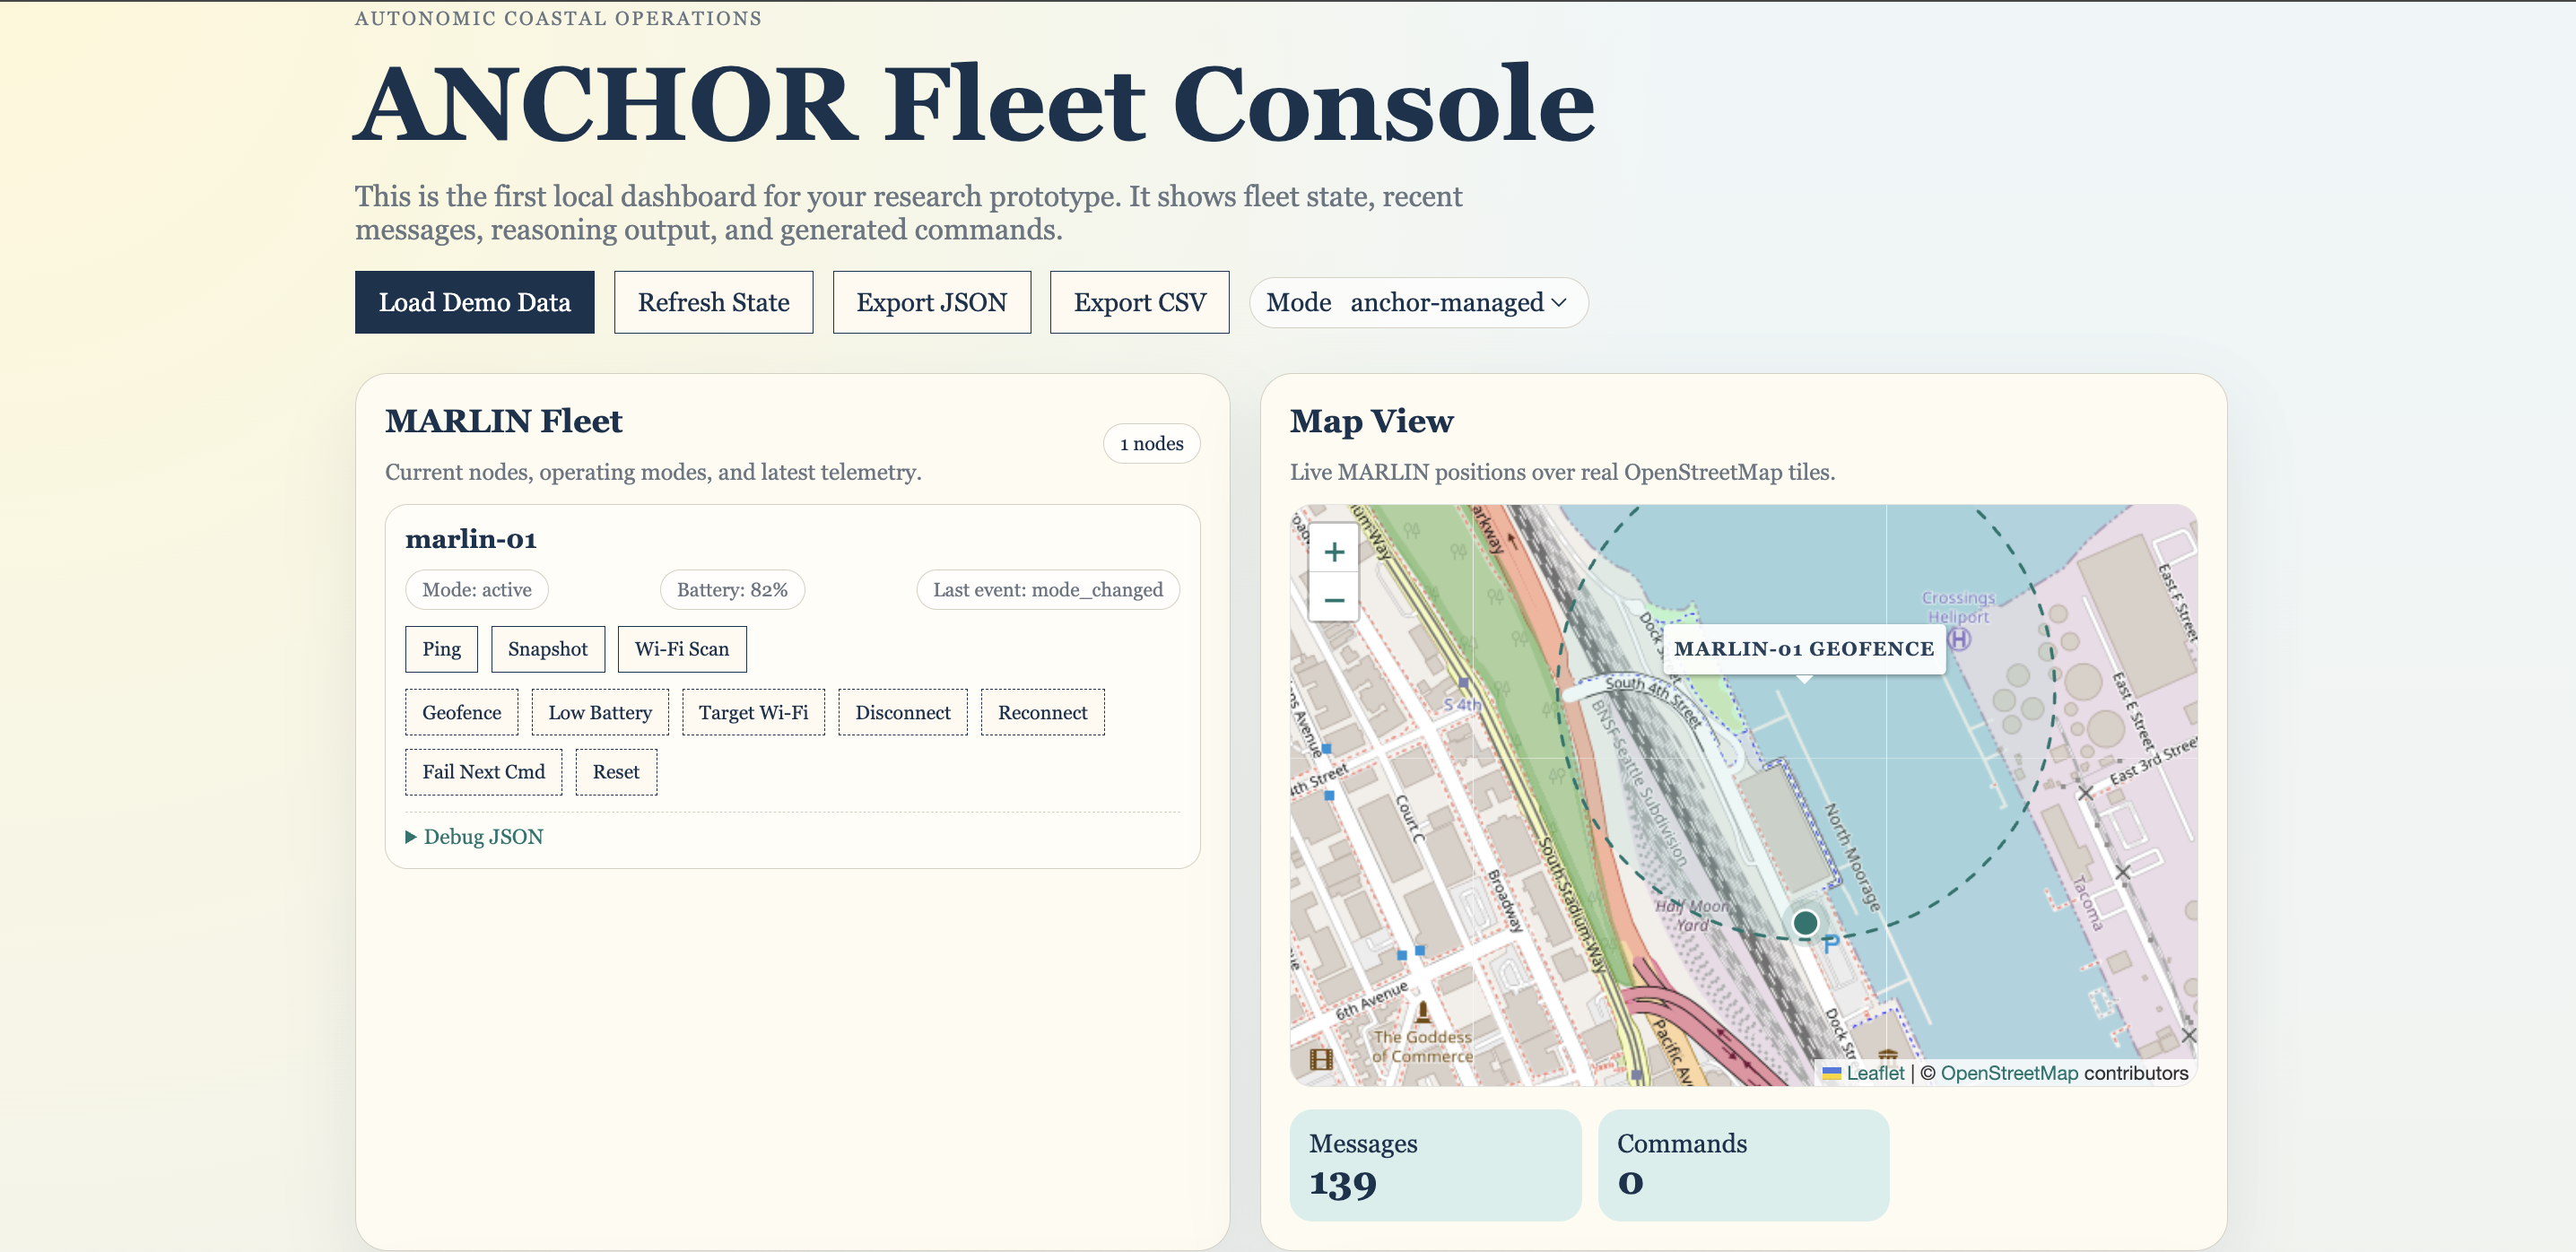
\includegraphics[width=0.48\textwidth]{images/web ui 1.png}
\caption{ANCHOR fleet and map view showing MARLIN state, operator command controls, live map position, and geofence context.}
\label{fig:dashboard-fleet-map}
\end{center}
\end{figure}

\begin{figure}[H]
\begin{center}
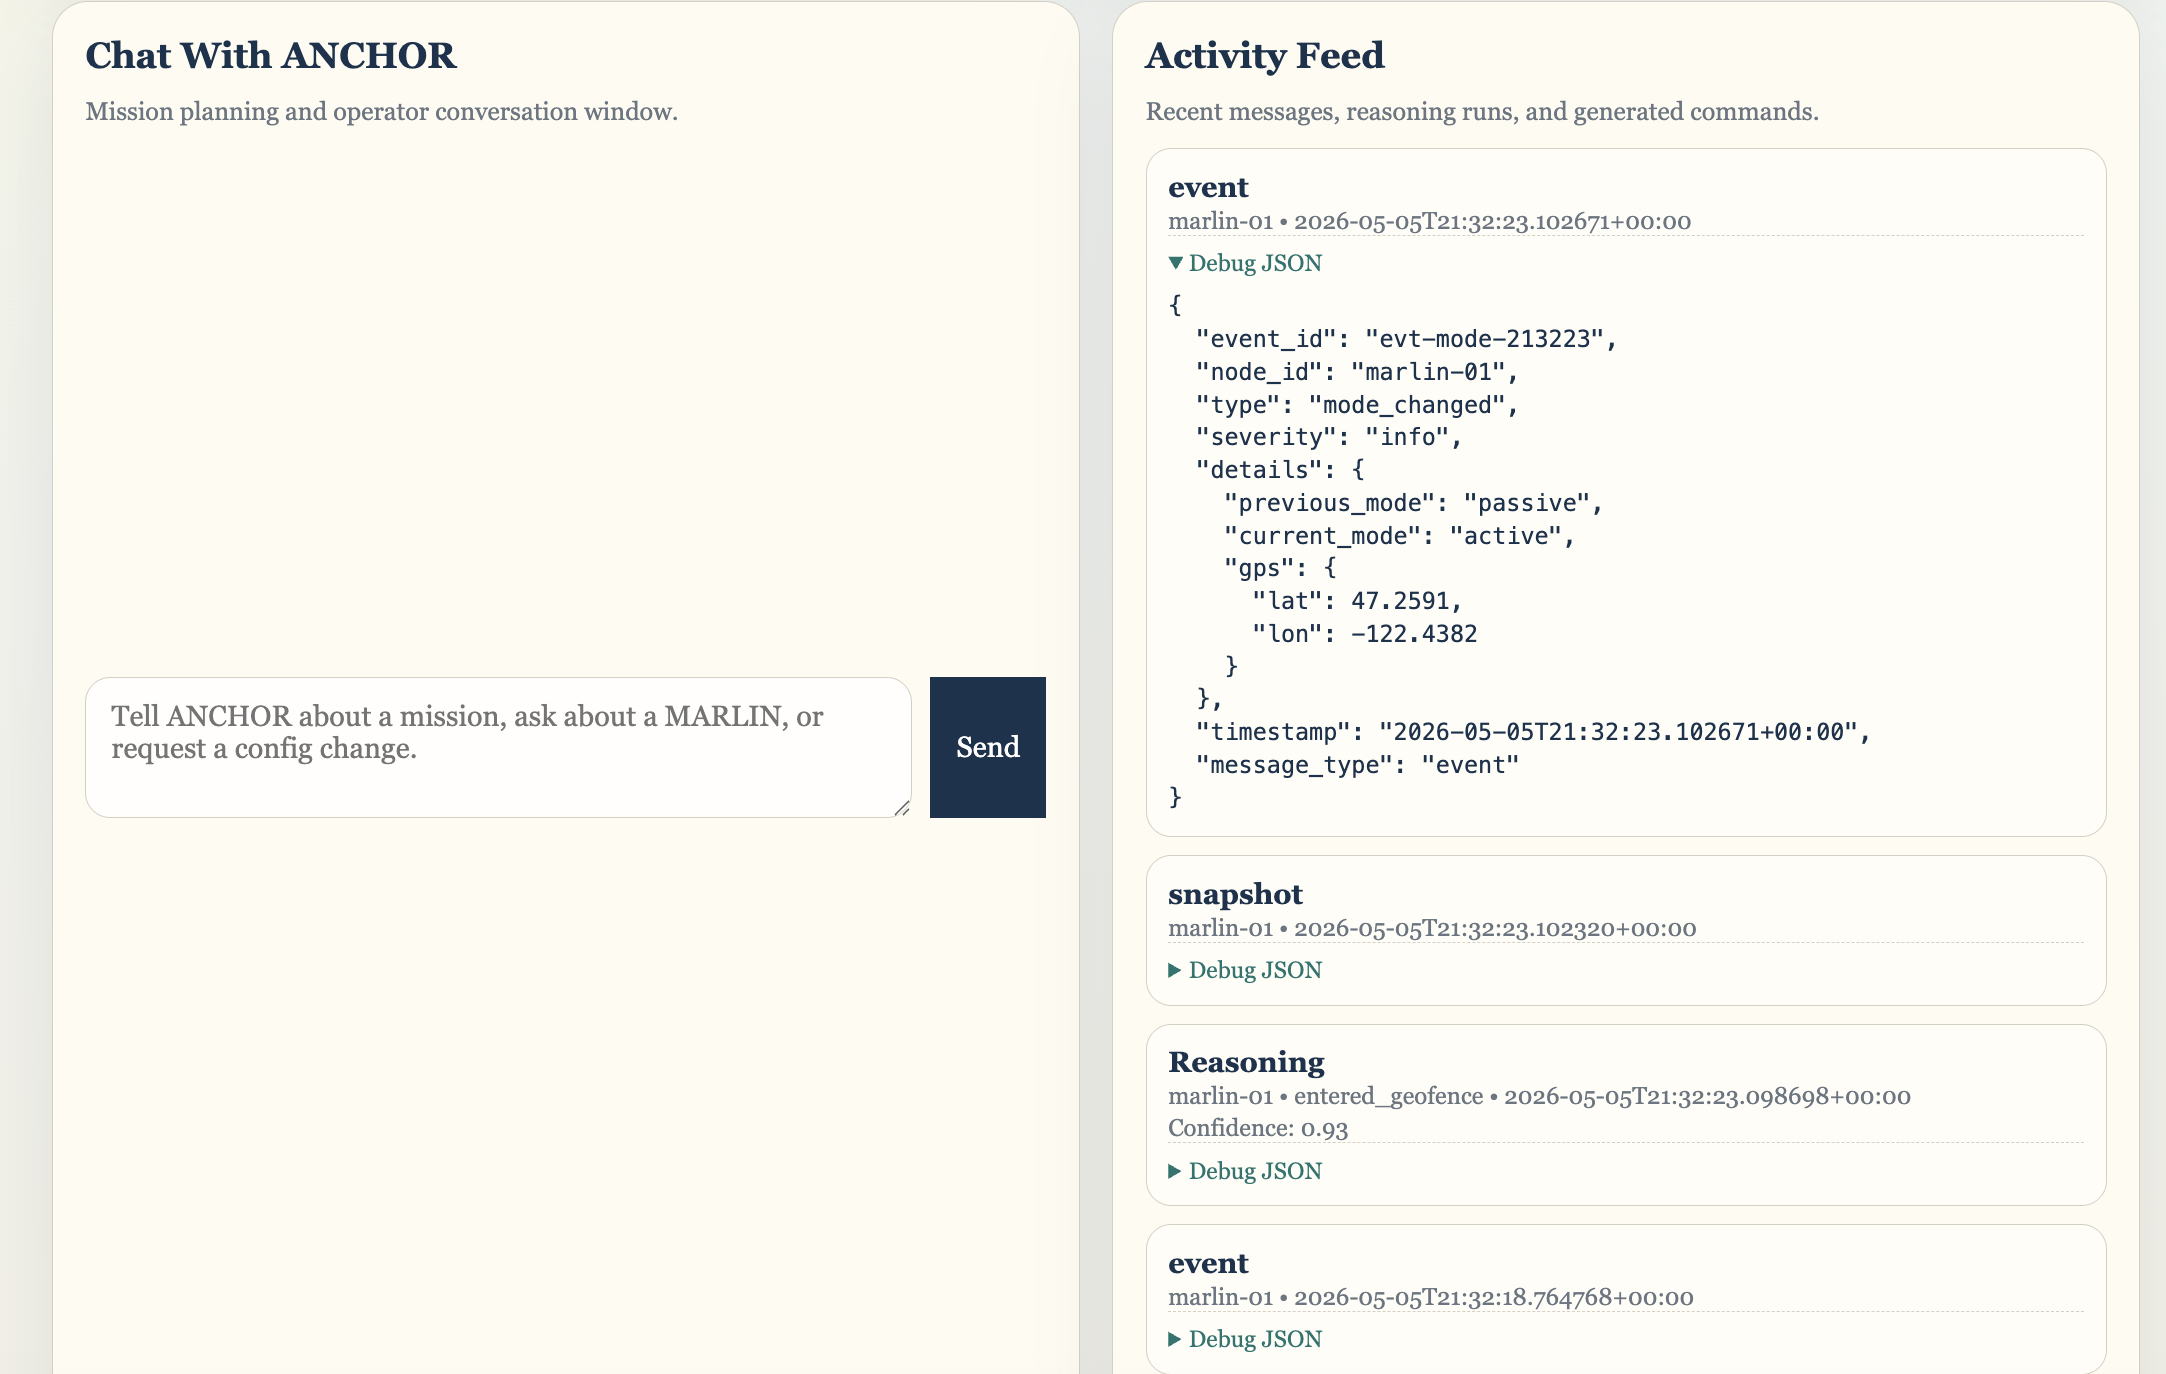
\includegraphics[width=0.48\textwidth]{images/web ui 2.png}
\caption{ANCHOR operator chat and activity feed showing event, snapshot, and reasoning records with expandable JSON details.}
\label{fig:dashboard-activity-feed}
\end{center}
\end{figure}

\begin{figure}[H]
\begin{center}
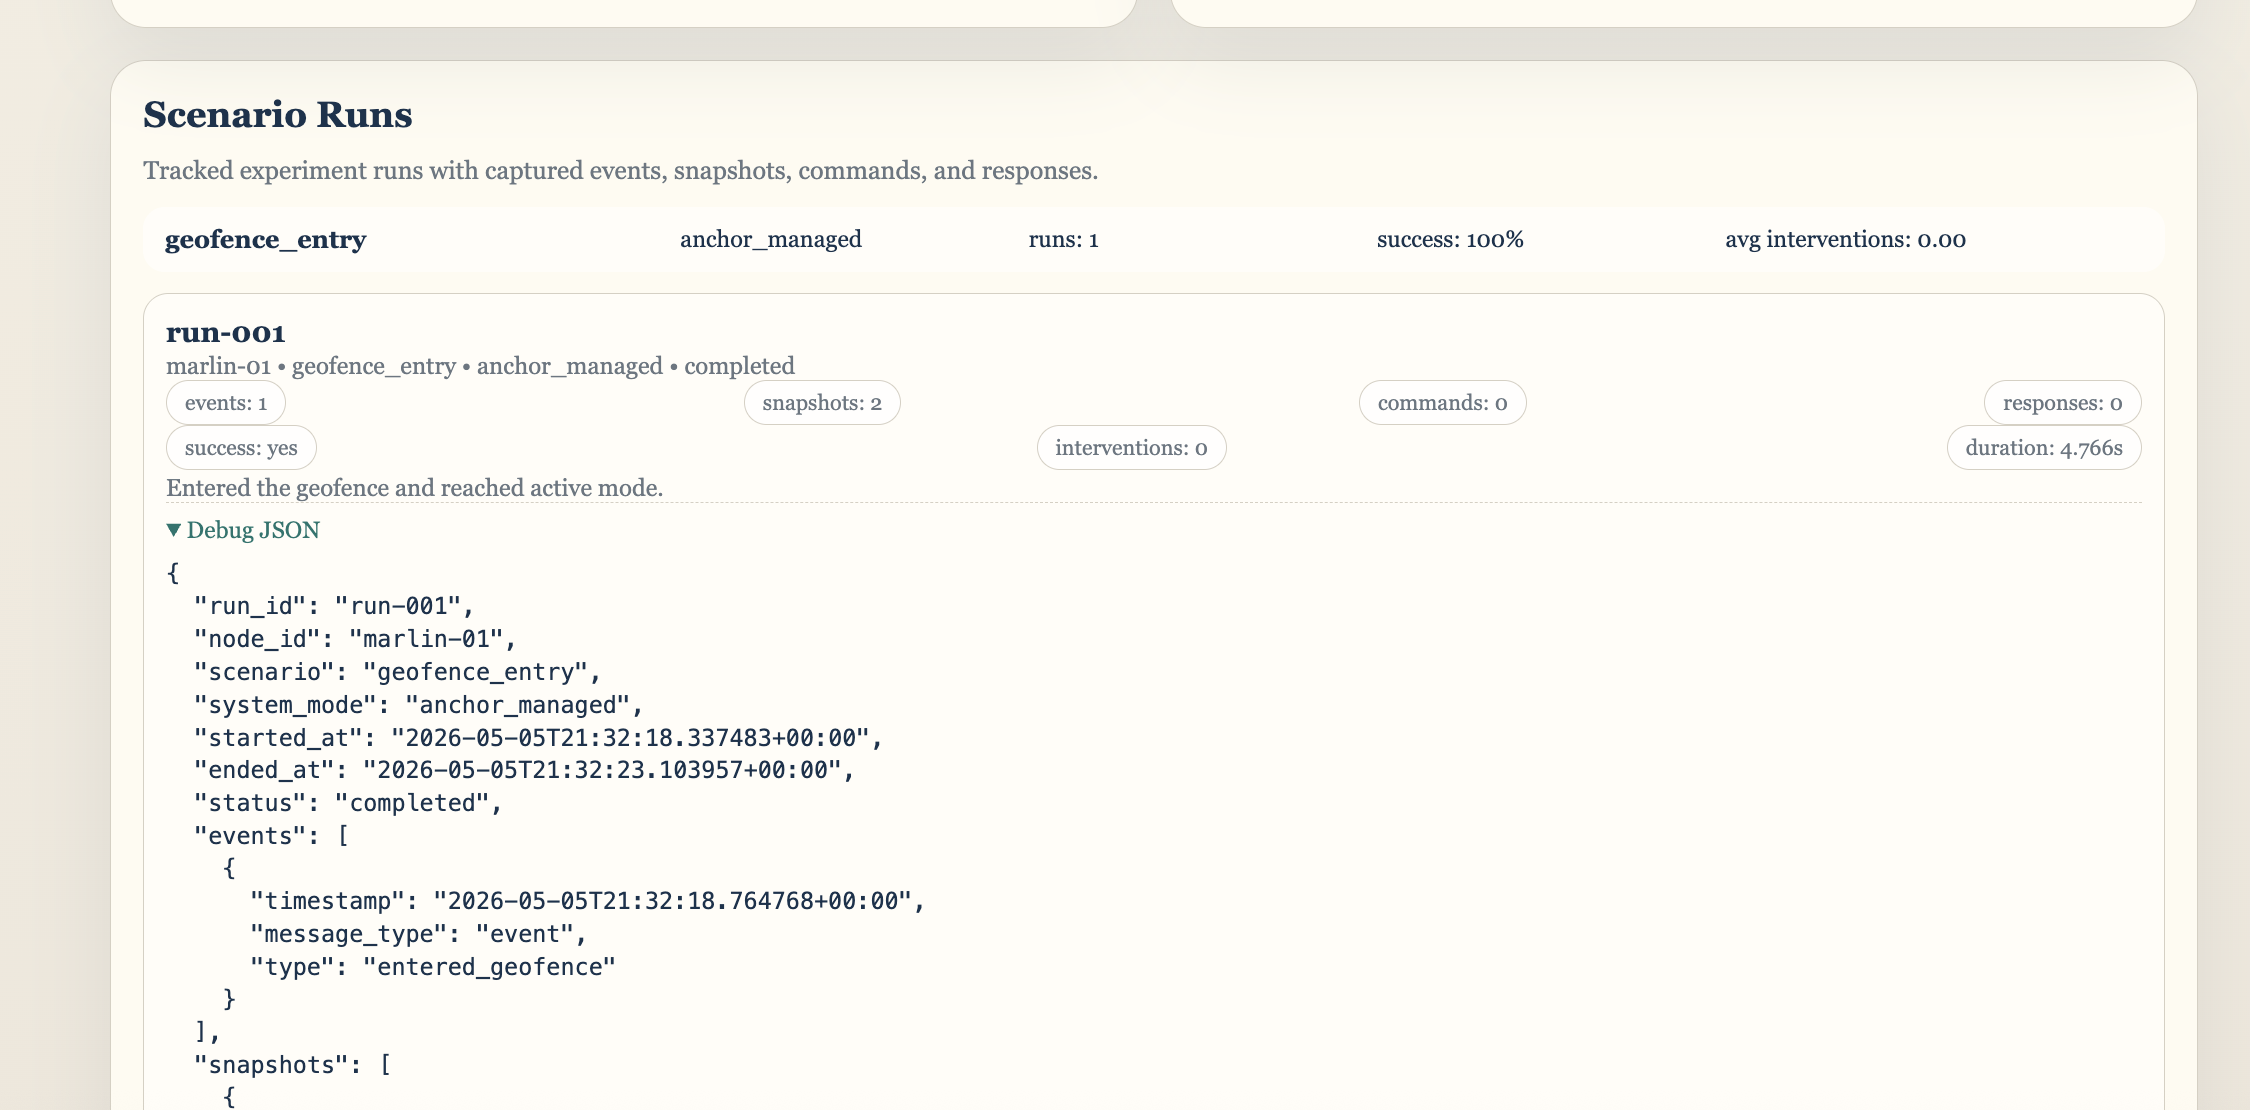
\includegraphics[width=0.48\textwidth]{images/web ui 3.png}
\caption{ANCHOR scenario-run panel used to summarize controlled experiment runs, including success status, intervention count, duration, and captured run data.}
\label{fig:dashboard-scenario-runs}
\end{center}
\end{figure}


\subsection{Execution Model and Autonomy Boundary}
The software stack reflects a deliberate boundary between reasoning and execution. Codex is used by ANCHOR as an analyze-and-plan engine, but it does not directly execute arbitrary shell commands on MARLIN nodes. Instead, it can only recommend actions from a predefined structured command set, and those recommendations must pass validation before they are issued.

This boundary is one of the most important results of the implementation. The original project vision implied a stronger form of decentralized agentic autonomy, but the codebase demonstrates that a more realistic and safer design is one in which LLM reasoning is mediated through explicit schemas, policy checks, and limited execution handlers. Thus, the software stack itself embodies the paper's transition from intended architecture to realized architecture.

\subsection{Current Prototype Scope}
The present implementation is intentionally a prototype rather than a production system. Several components are simulated or simplified, including sensor inputs, node-to-base communication, and persistent storage. Despite this, the current software stack is sufficient to validate the central architectural claims of the project. MARLIN can act as a mission-aware edge node, ANCHOR can function as a reasoning-enabled base station, and Codex can participate in the autonomic loop without requiring unrestricted control over remote machines.

In that sense, the software stack is not just an implementation detail of the project, it allows me to test the research question.

\subsection{Source Code Availability}
The prototype source code for ANCHOR and MARLIN is available at:
\url{https://github.com/Sajivv/anchor}

\section{Results and Validation}~\label{results}
To validate that ANCHOR functions as an effective autonomic manager, the prototype was evaluated against core autonomic properties adapted to the realized hybrid architecture.

\textbf{Self-Configuration:} MARLIN should begin operating from an assigned mission configuration without repeated manual intervention. ANCHOR should be able to define geofence-driven mission behavior, reporting cadence, and Wi-Fi scanning policy.

\textbf{Self-Healing:} ANCHOR and MARLIN together should detect and recover from failures such as command failure, communication interruption, or sensor-related anomalies. If ANCHOR becomes unreachable, MARLIN should continue operating from cached mission policy and resume synchronization later.

\textbf{Self-Optimization:} The system should adapt reporting and scan behavior based on mission state. A MARLIN outside a target geofence should remain passive, while a MARLIN inside the target region should increase activity and begin Wi-Fi scanning.

\textbf{Self-Protection:} The system should restrict expensive or risky activity when conditions require it, especially under low battery conditions. In the realized prototype, this includes entering low-power mode and suppressing mission-driven scanning behavior when battery constraints become severe.

\subsection{Human Monitoring Reduction}
The primary quantitative target for this project was a 65\% reduction in required human monitoring effort compared to a baseline system without ANCHOR. Based on the completed scenario matrix, the baseline runs required a total of five operator interventions, while the ANCHOR-managed runs required a total of one operator intervention.

Let $B$ represent baseline interventions and $A$ represent ANCHOR-managed interventions. The reduction is calculated as:

\begin{equation}
    R = \frac{B - A}{B} \times 100
\end{equation}

Substituting the observed totals gives:

\begin{equation}
    R = \frac{5 - 1}{5} \times 100 = 80\%
\end{equation}

This exceeds the stated success criterion of 65\% and shows that the realized hybrid architecture substantially reduces operator burden, even though some categories of failure handling remain incomplete.

\subsection{LLM Resource Usage and Cost}
Because ANCHOR uses Codex as part of the analyze-and-plan loop, the prototype also produced measurable LLM resource usage. The OpenAI usage export for the project window from April 5, 2026 through May 5, 2026 recorded 16 model requests using \texttt{gpt-5.3-codex}. Across those requests, the system used 4,995 input tokens and 3,028 output tokens, for a total of 8,023 tokens.

The corresponding cost export reported a total cost of approximately \$0.05 USD for those requests. This low observed cost is partly due to the limited scale of the prototype and the small number of reasoning-triggering events, but it is still useful because it shows that the ANCHOR-managed behavior tested in this project did not require a large amount of LLM usage. In a larger fleet deployment, the same measurement would need to be repeated with more nodes, longer missions, and more frequent reasoning triggers.

\begin{figure}[H]
\begin{center}
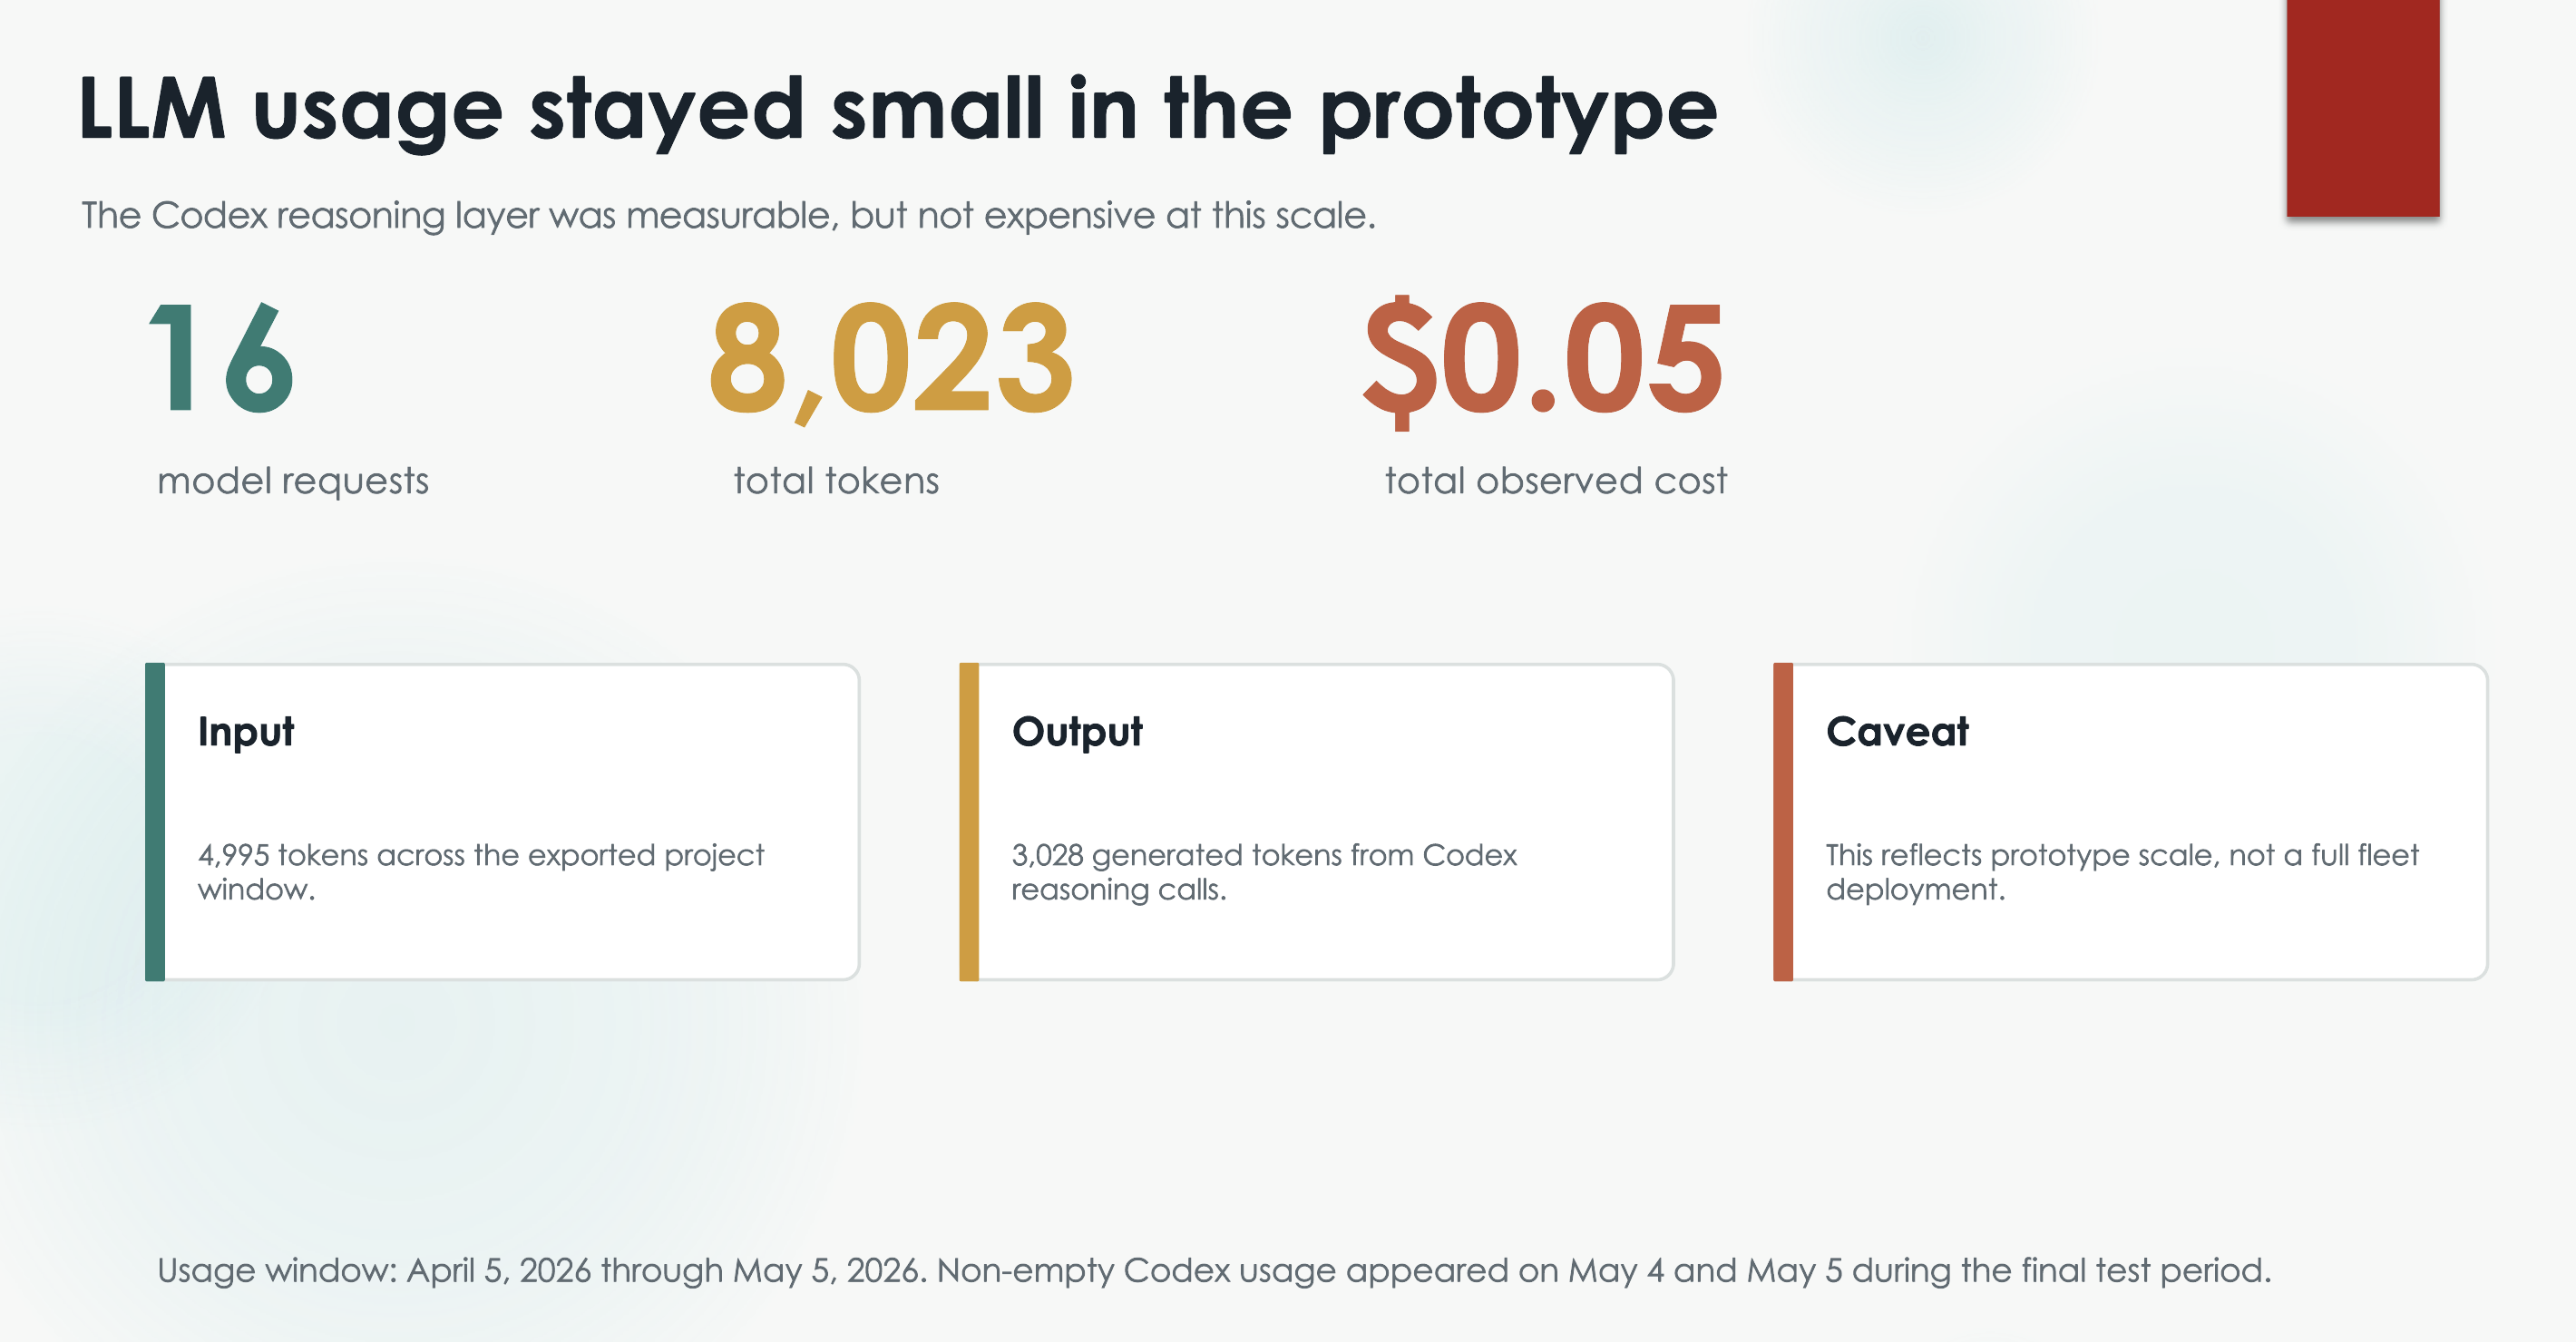
\includegraphics[width=0.48\textwidth]{images/llm usage.png}
\caption{Overview of LLM Usage}
\label{fig:dashboard-scenario-runs}
\end{center}
\end{figure}


\subsection{Evaluation Scenarios}
The prototype was designed around five controlled scenarios, each intended to compare a baseline configuration against an ANCHOR-managed configuration:

\begin{itemize}
    \item \textbf{Geofence Entry:} Whether the node correctly transitions from passive to active behavior when crossing into the mission area.
    \item \textbf{Low Battery Condition:} Whether the node reduces activity and preserves energy when battery state falls below threshold.
    \item \textbf{Target Wi-Fi Detection:} Whether the system can move from observation of a mission-relevant wireless target to a useful follow-up action.
    \item \textbf{Loss of Connectivity to ANCHOR:} Whether MARLIN continues operating from cached mission policy and later resumes synchronization.
    \item \textbf{Command Failure:} Whether a failed remote action is detected and whether ANCHOR can respond with retry, alternate action, or escalation.
\end{itemize}

These controlled scenarios remain important because they provide repeatable baseline-versus-managed comparisons and allow intervention counts, command outcomes, and scenario completion to be measured under known conditions.

\subsection{Controlled Scenario Results}
All five scenarios were exercised in both baseline and ANCHOR-managed configurations. Table~\ref{tab:scenario-results} summarizes the completed runs.

\begin{table}[H]
\caption{Controlled Scenario Results}
\label{tab:scenario-results}
\begin{center}
\footnotesize
\setlength{\tabcolsep}{3pt}
\begin{tabularx}{\columnwidth}{|p{0.18\columnwidth}|p{0.19\columnwidth}|c|c|X|}
\hline
Scenario & Mode & Success & Interventions & Notes \\
\hline
Low Battery & Baseline & Yes & 1 & Operator reduced activity manually \\
Low Battery & ANCHOR-managed & Yes & 0 & Local low-power transition, no follow-up needed \\
Geofence Entry & Baseline & Yes & 1 & Operator would need to start mission activity \\
Geofence Entry & ANCHOR-managed & Yes & 0 & Automatic active-mode transition and scan behavior \\
Target Wi-Fi Detection & Baseline & Yes & 1 & Operator must interpret detection \\
Target Wi-Fi Detection & ANCHOR-managed & Yes & 0 & Detection captured without operator action \\
Disconnect & Baseline & No & 1 & Recovery required operator verification \\
Disconnect & ANCHOR-managed & No & 0 & Local continuity preserved, sync resumed after reconnect \\
Command Failure & Baseline & No & 1 & Operator manually marked failure \\
Command Failure & ANCHOR-managed & No & 1 & Managed mode did not improve failure observability \\
\hline
\end{tabularx}
\end{center}
\end{table}

Three patterns stand out from these controlled runs. First, ANCHOR-managed mode consistently reduced intervention count in low battery, geofence entry, and target Wi-Fi detection. Second, disconnect handling demonstrated graceful degradation and later recovery, but not true autonomous reestablishment of the underlying link. Third, command-failure handling remains a significant limitation of the current prototype, because neither baseline nor ANCHOR-managed mode reliably surfaced a failed command response back into the experiment harness.

\begin{figure}[H]
\begin{center}
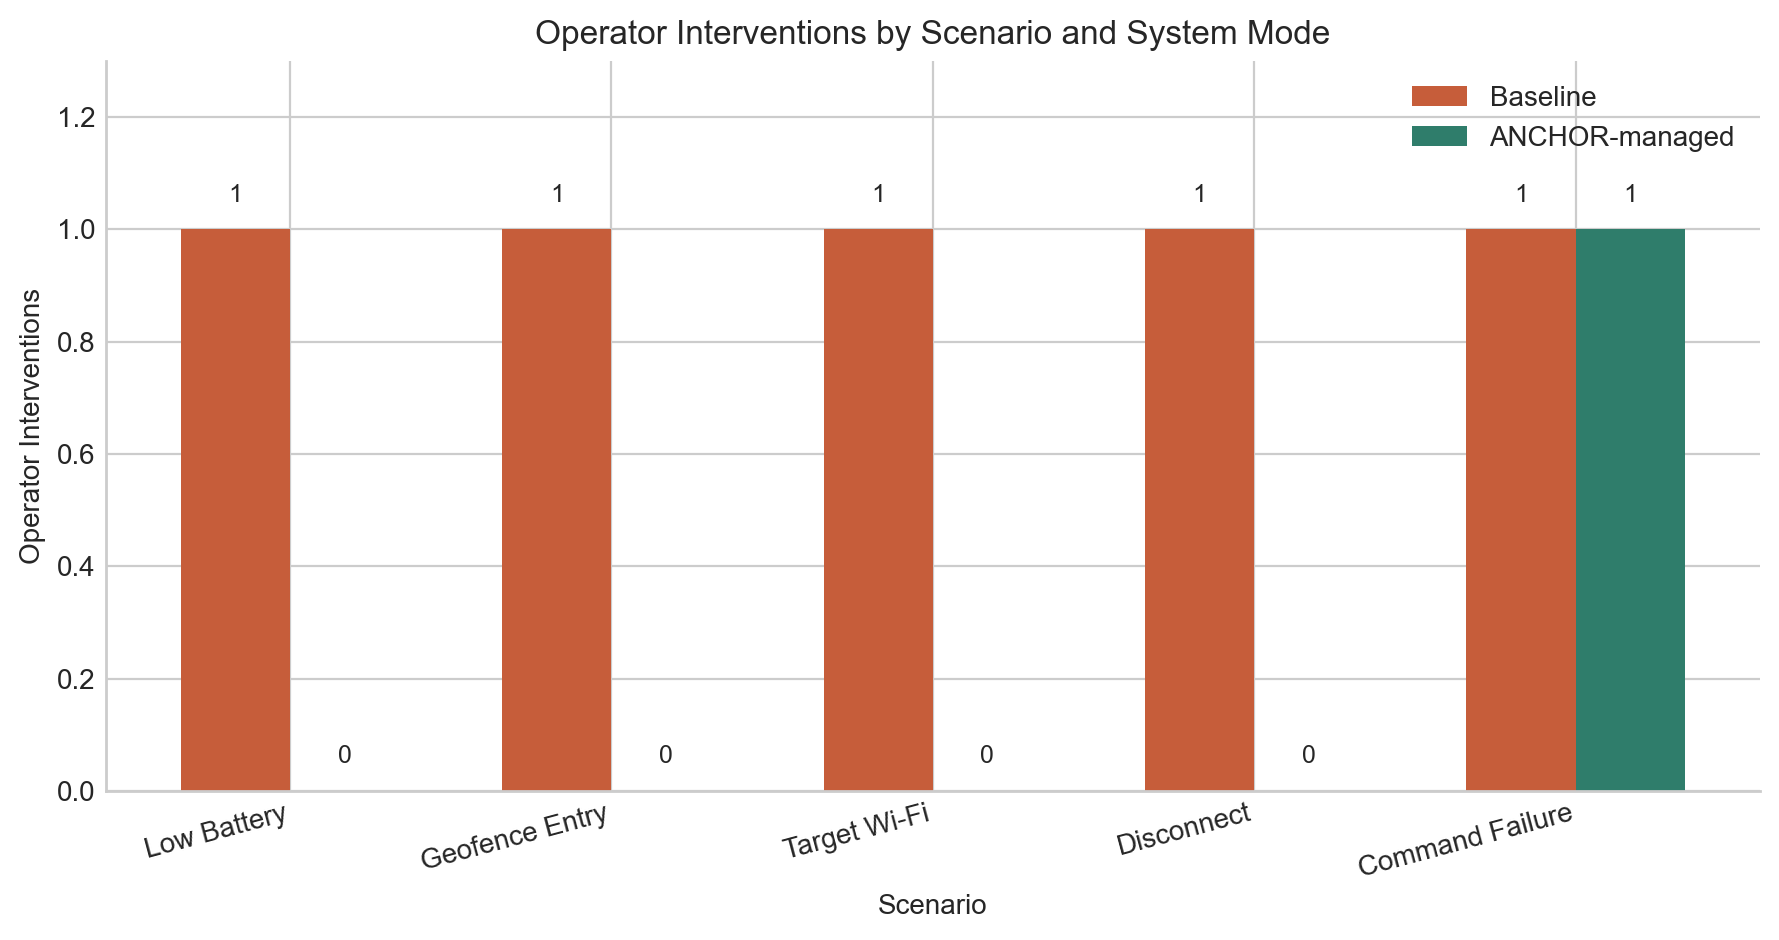
\includegraphics[width=0.48\textwidth]{images/intervention_bar_chart.png}
\caption{Operator interventions required in each controlled scenario for the baseline and ANCHOR-managed configurations.}
\label{fig:intervention-bar-chart}
\end{center}
\end{figure}

\subsection{Live Field Test in Tacoma Foss Harbor}
To complement the controlled mock-data scenarios, a live field test was conducted in Tacoma's Foss Harbor using a two-machine deployment. ANCHOR ran on a MacBook Pro acting as the base station, while MARLIN ran on an Ubuntu laptop acting as the remote node. Both systems were connected through a mobile Wi-Fi hotspot so that they could exchange telemetry and commands. The hotspot also provided a live GPS NMEA stream to MARLIN, allowing the node to report real position updates to ANCHOR at one-minute intervals. MARLIN additionally reported the Ubuntu laptop's battery percentage to ANCHOR.

\begin{figure*}[t]
\begin{center}
\begin{minipage}{0.32\textwidth}
\centering
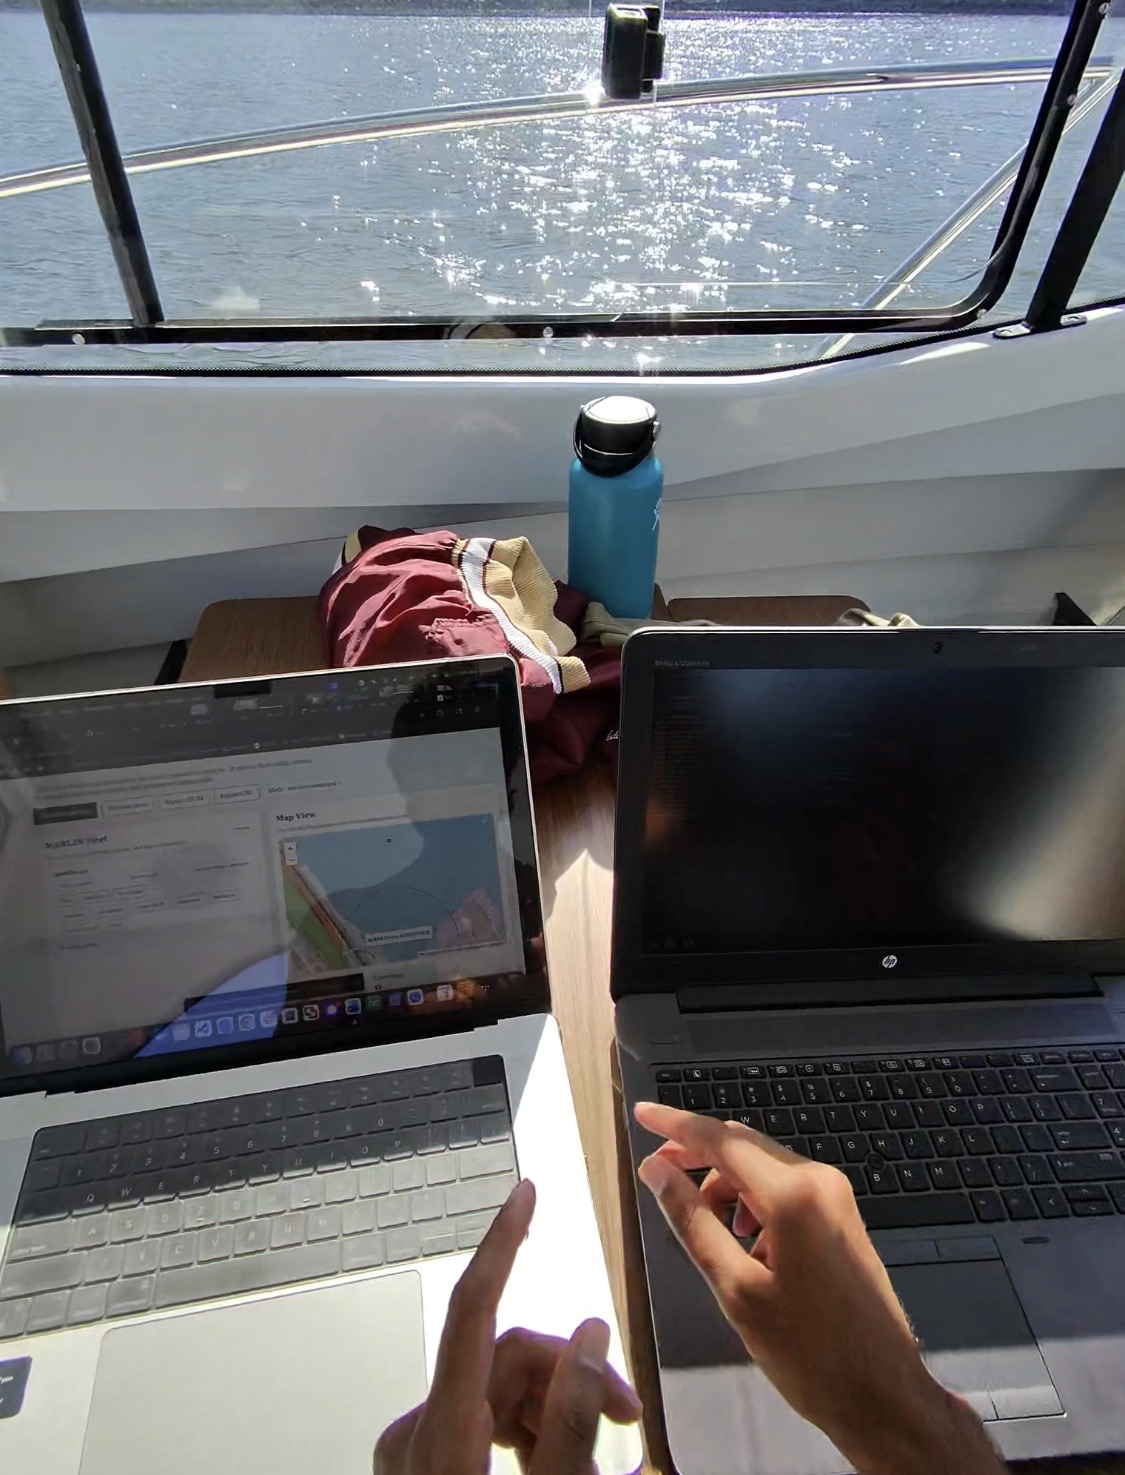
\includegraphics[width=\textwidth]{images/both laptops in boat.jpg}
\end{minipage}\hfill
\begin{minipage}{0.32\textwidth}
\centering
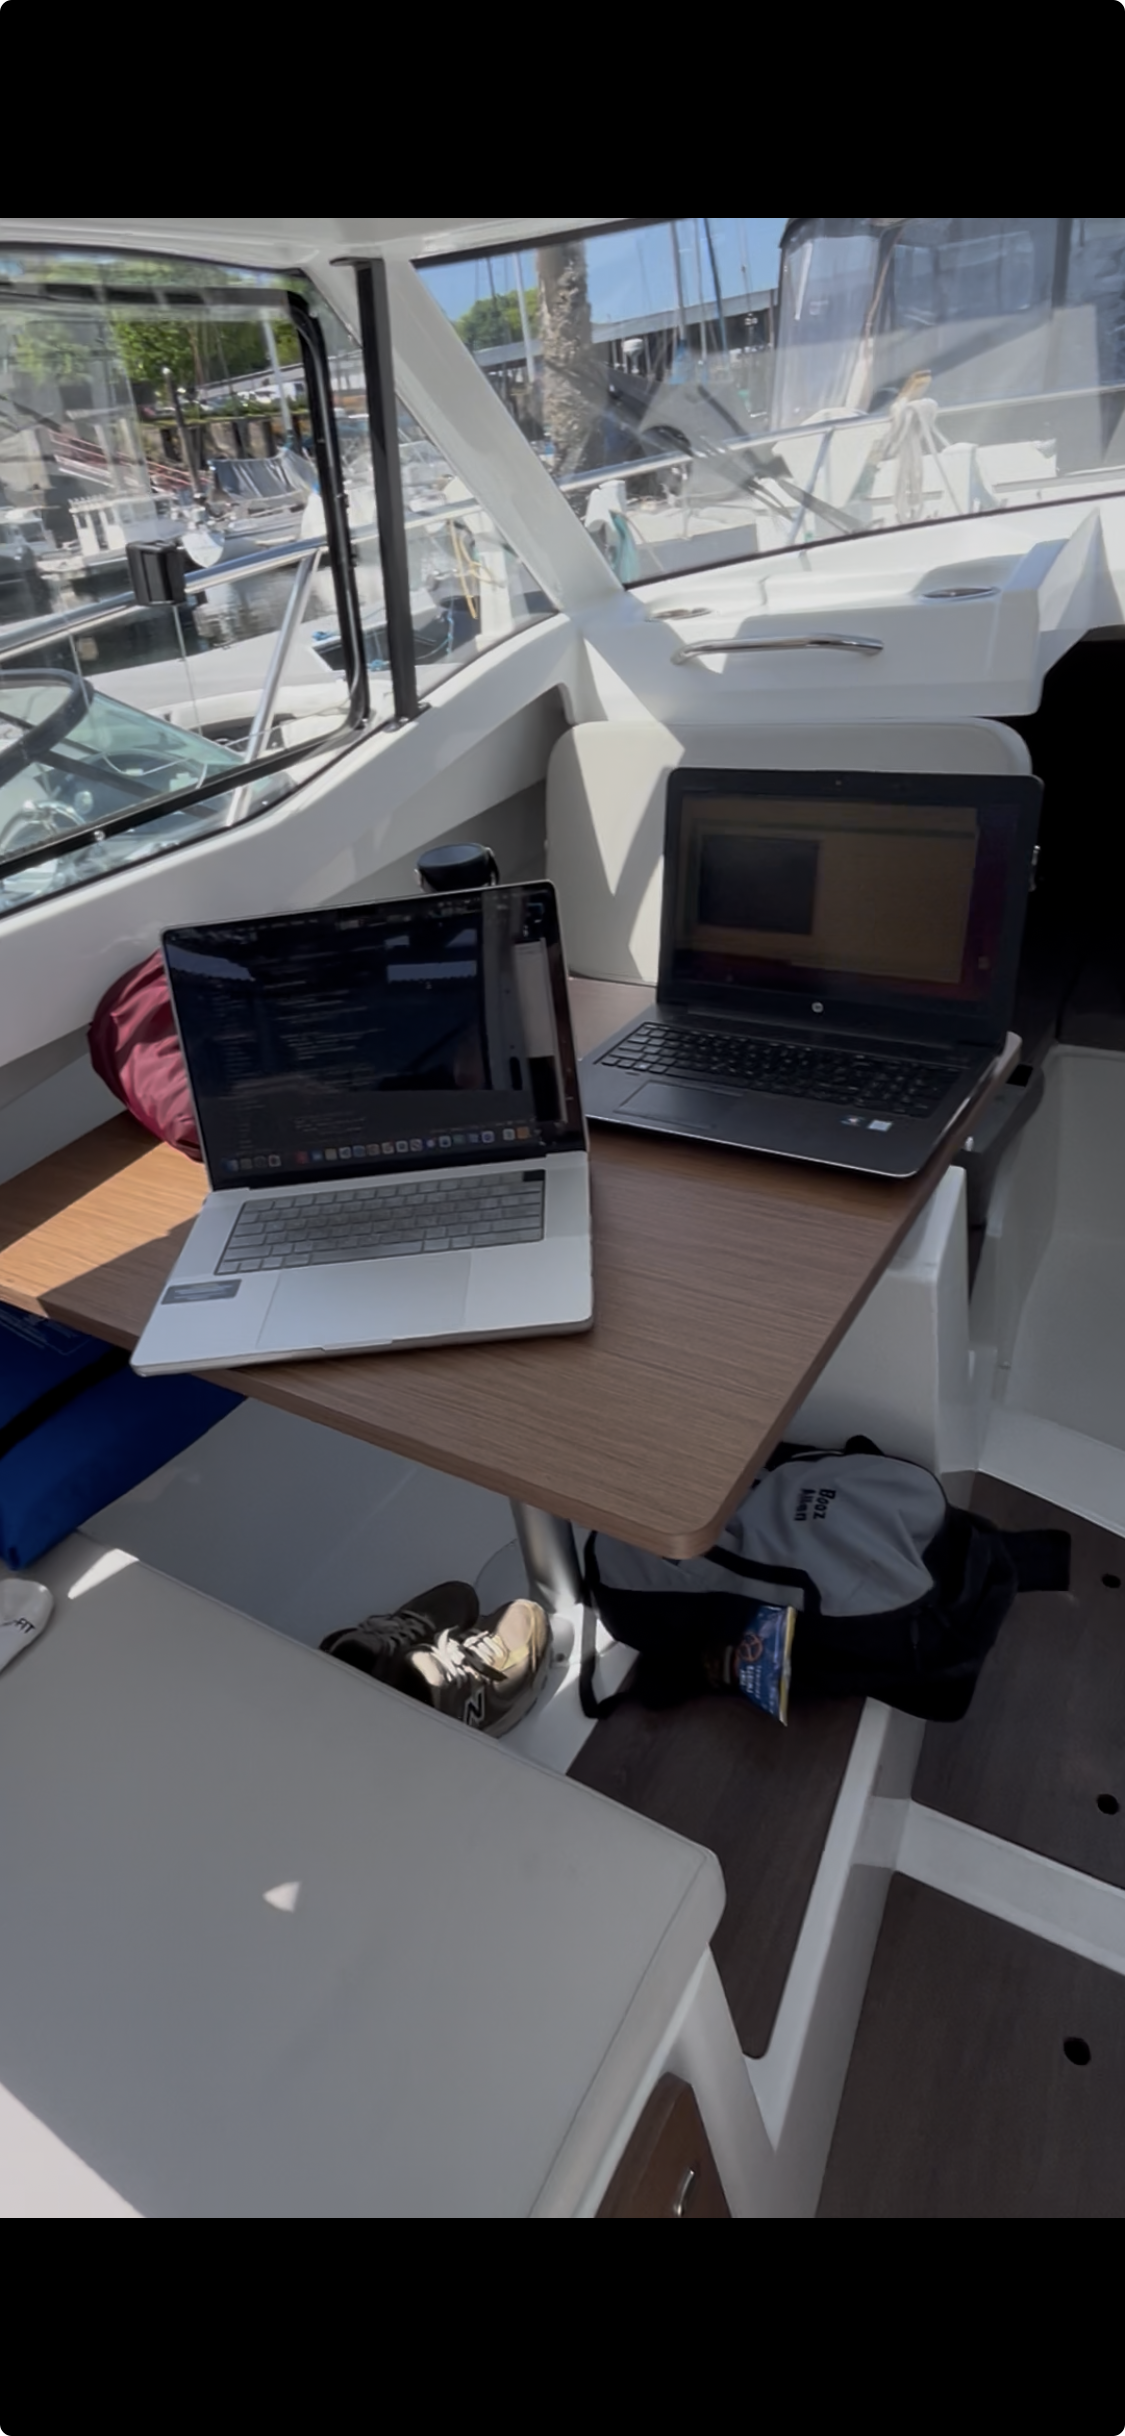
\includegraphics[width=\textwidth]{images/Anchor base tation and marlin laptop.png}
\end{minipage}\hfill
\begin{minipage}{0.32\textwidth}
\centering
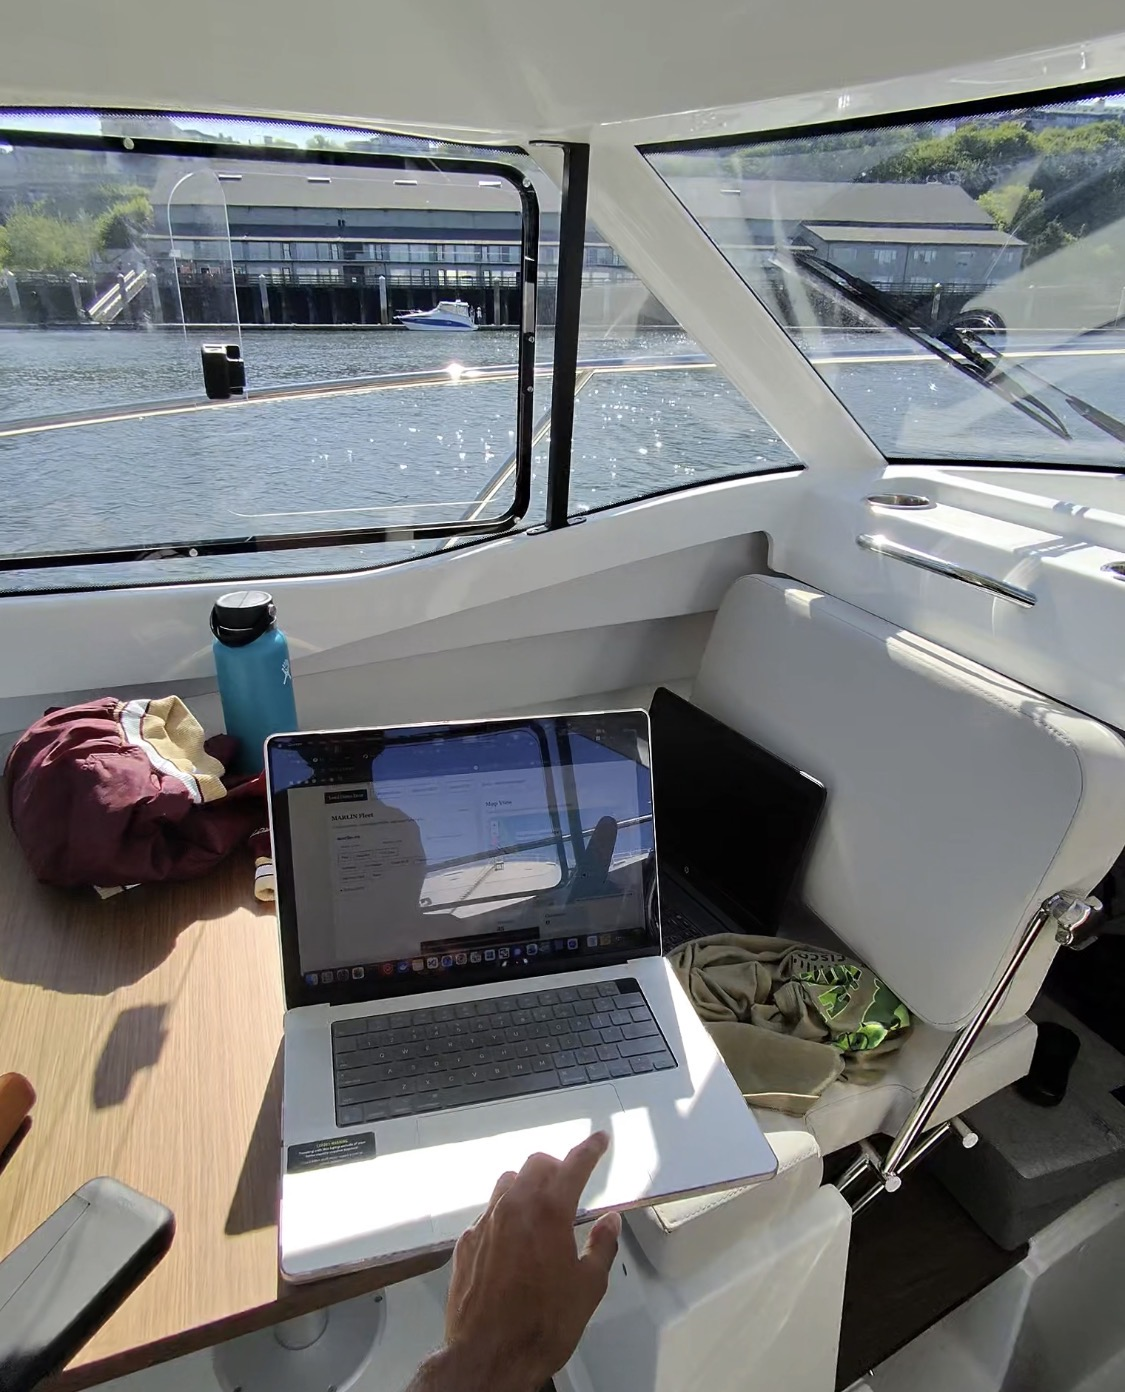
\includegraphics[width=\textwidth]{images/using anchor on boat.jpg}
\end{minipage}
\caption{Boat-based deployment views from the Tacoma field test. Left: the two-machine setup during the live run. Center: the MacBook ANCHOR base station and Ubuntu MARLIN laptop arranged aboard the vessel. Right: ANCHOR in active use during the on-water test.}
\label{fig:field-test-setup}
\end{center}
\end{figure*}

Testing began near Foss Harbor Marina with MARLIN outside the configured geofence and operating in passive mode. While outside the geofence, MARLIN transmitted periodic GPS snapshots to ANCHOR approximately once per minute, allowing the operator to observe real movement in the dashboard. As the vessel drifted toward the target area, ANCHOR was placed in ANCHOR-managed mode so that geofence entry would trigger the higher-order reasoning layer.

\begin{figure*}[t]
\begin{center}
\begin{minipage}{0.54\textwidth}
\centering
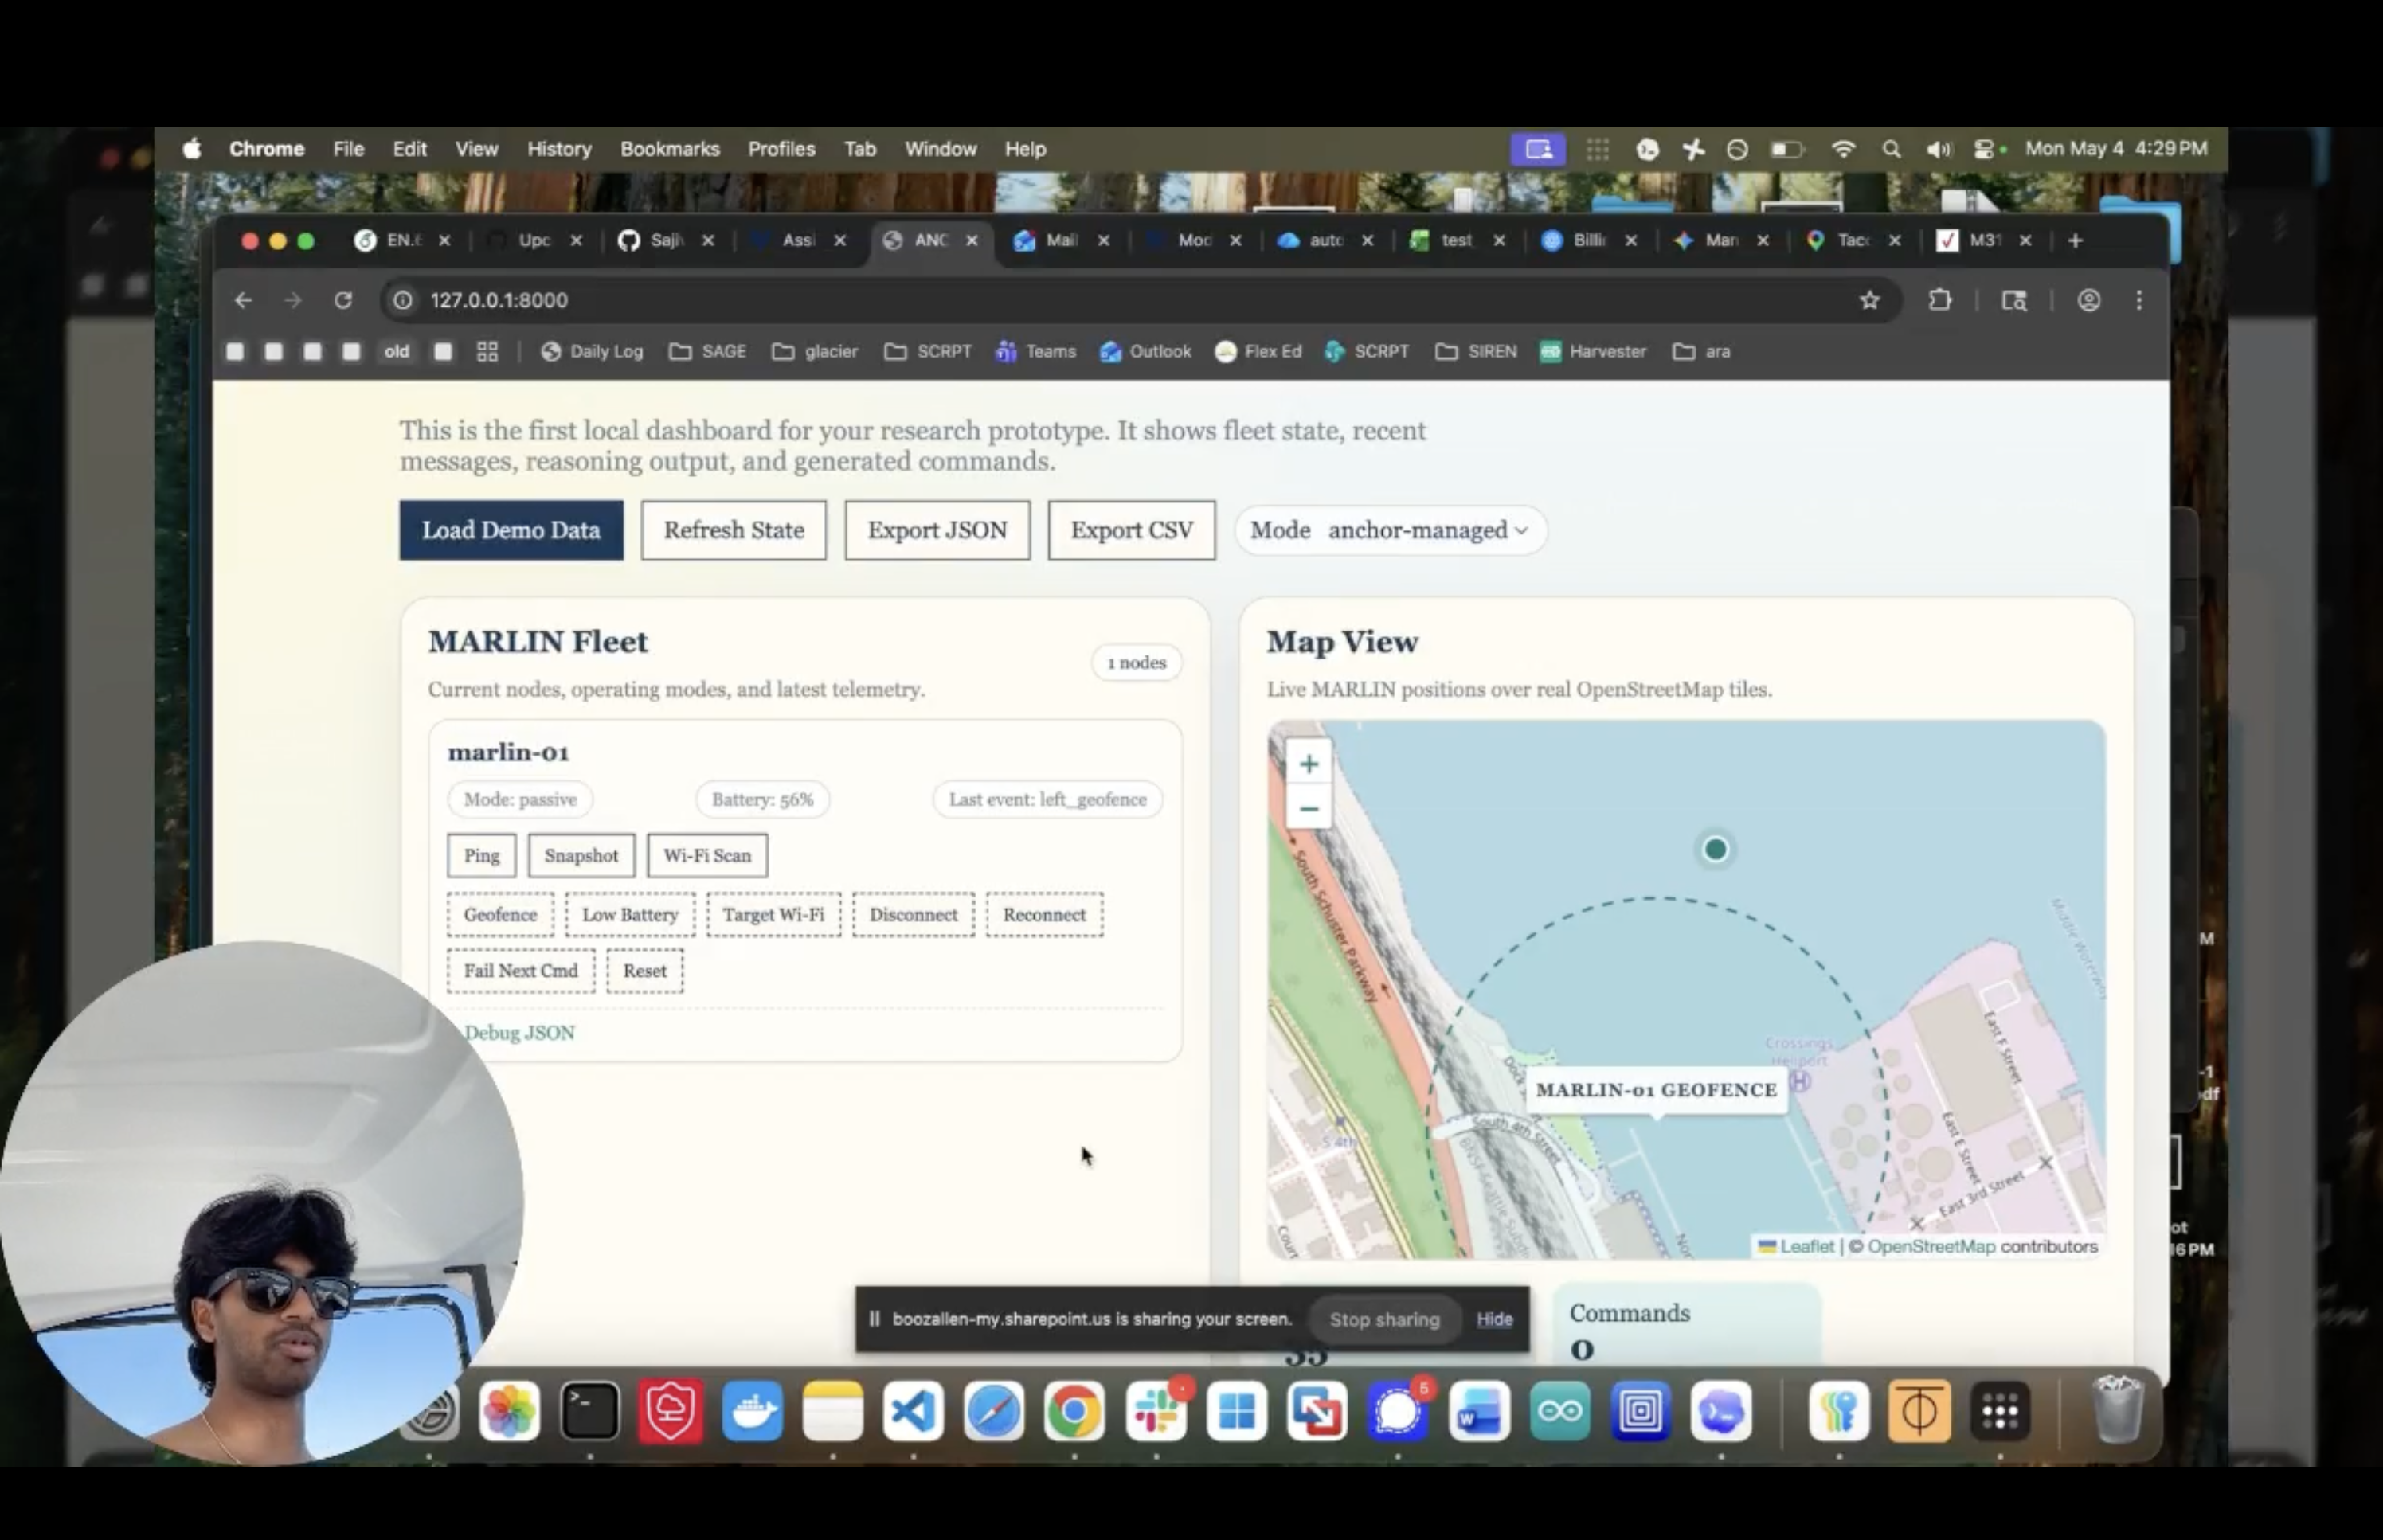
\includegraphics[width=\textwidth]{images/marlin outside geofence.png}
\end{minipage}\hfill
\begin{minipage}{0.42\textwidth}
\centering
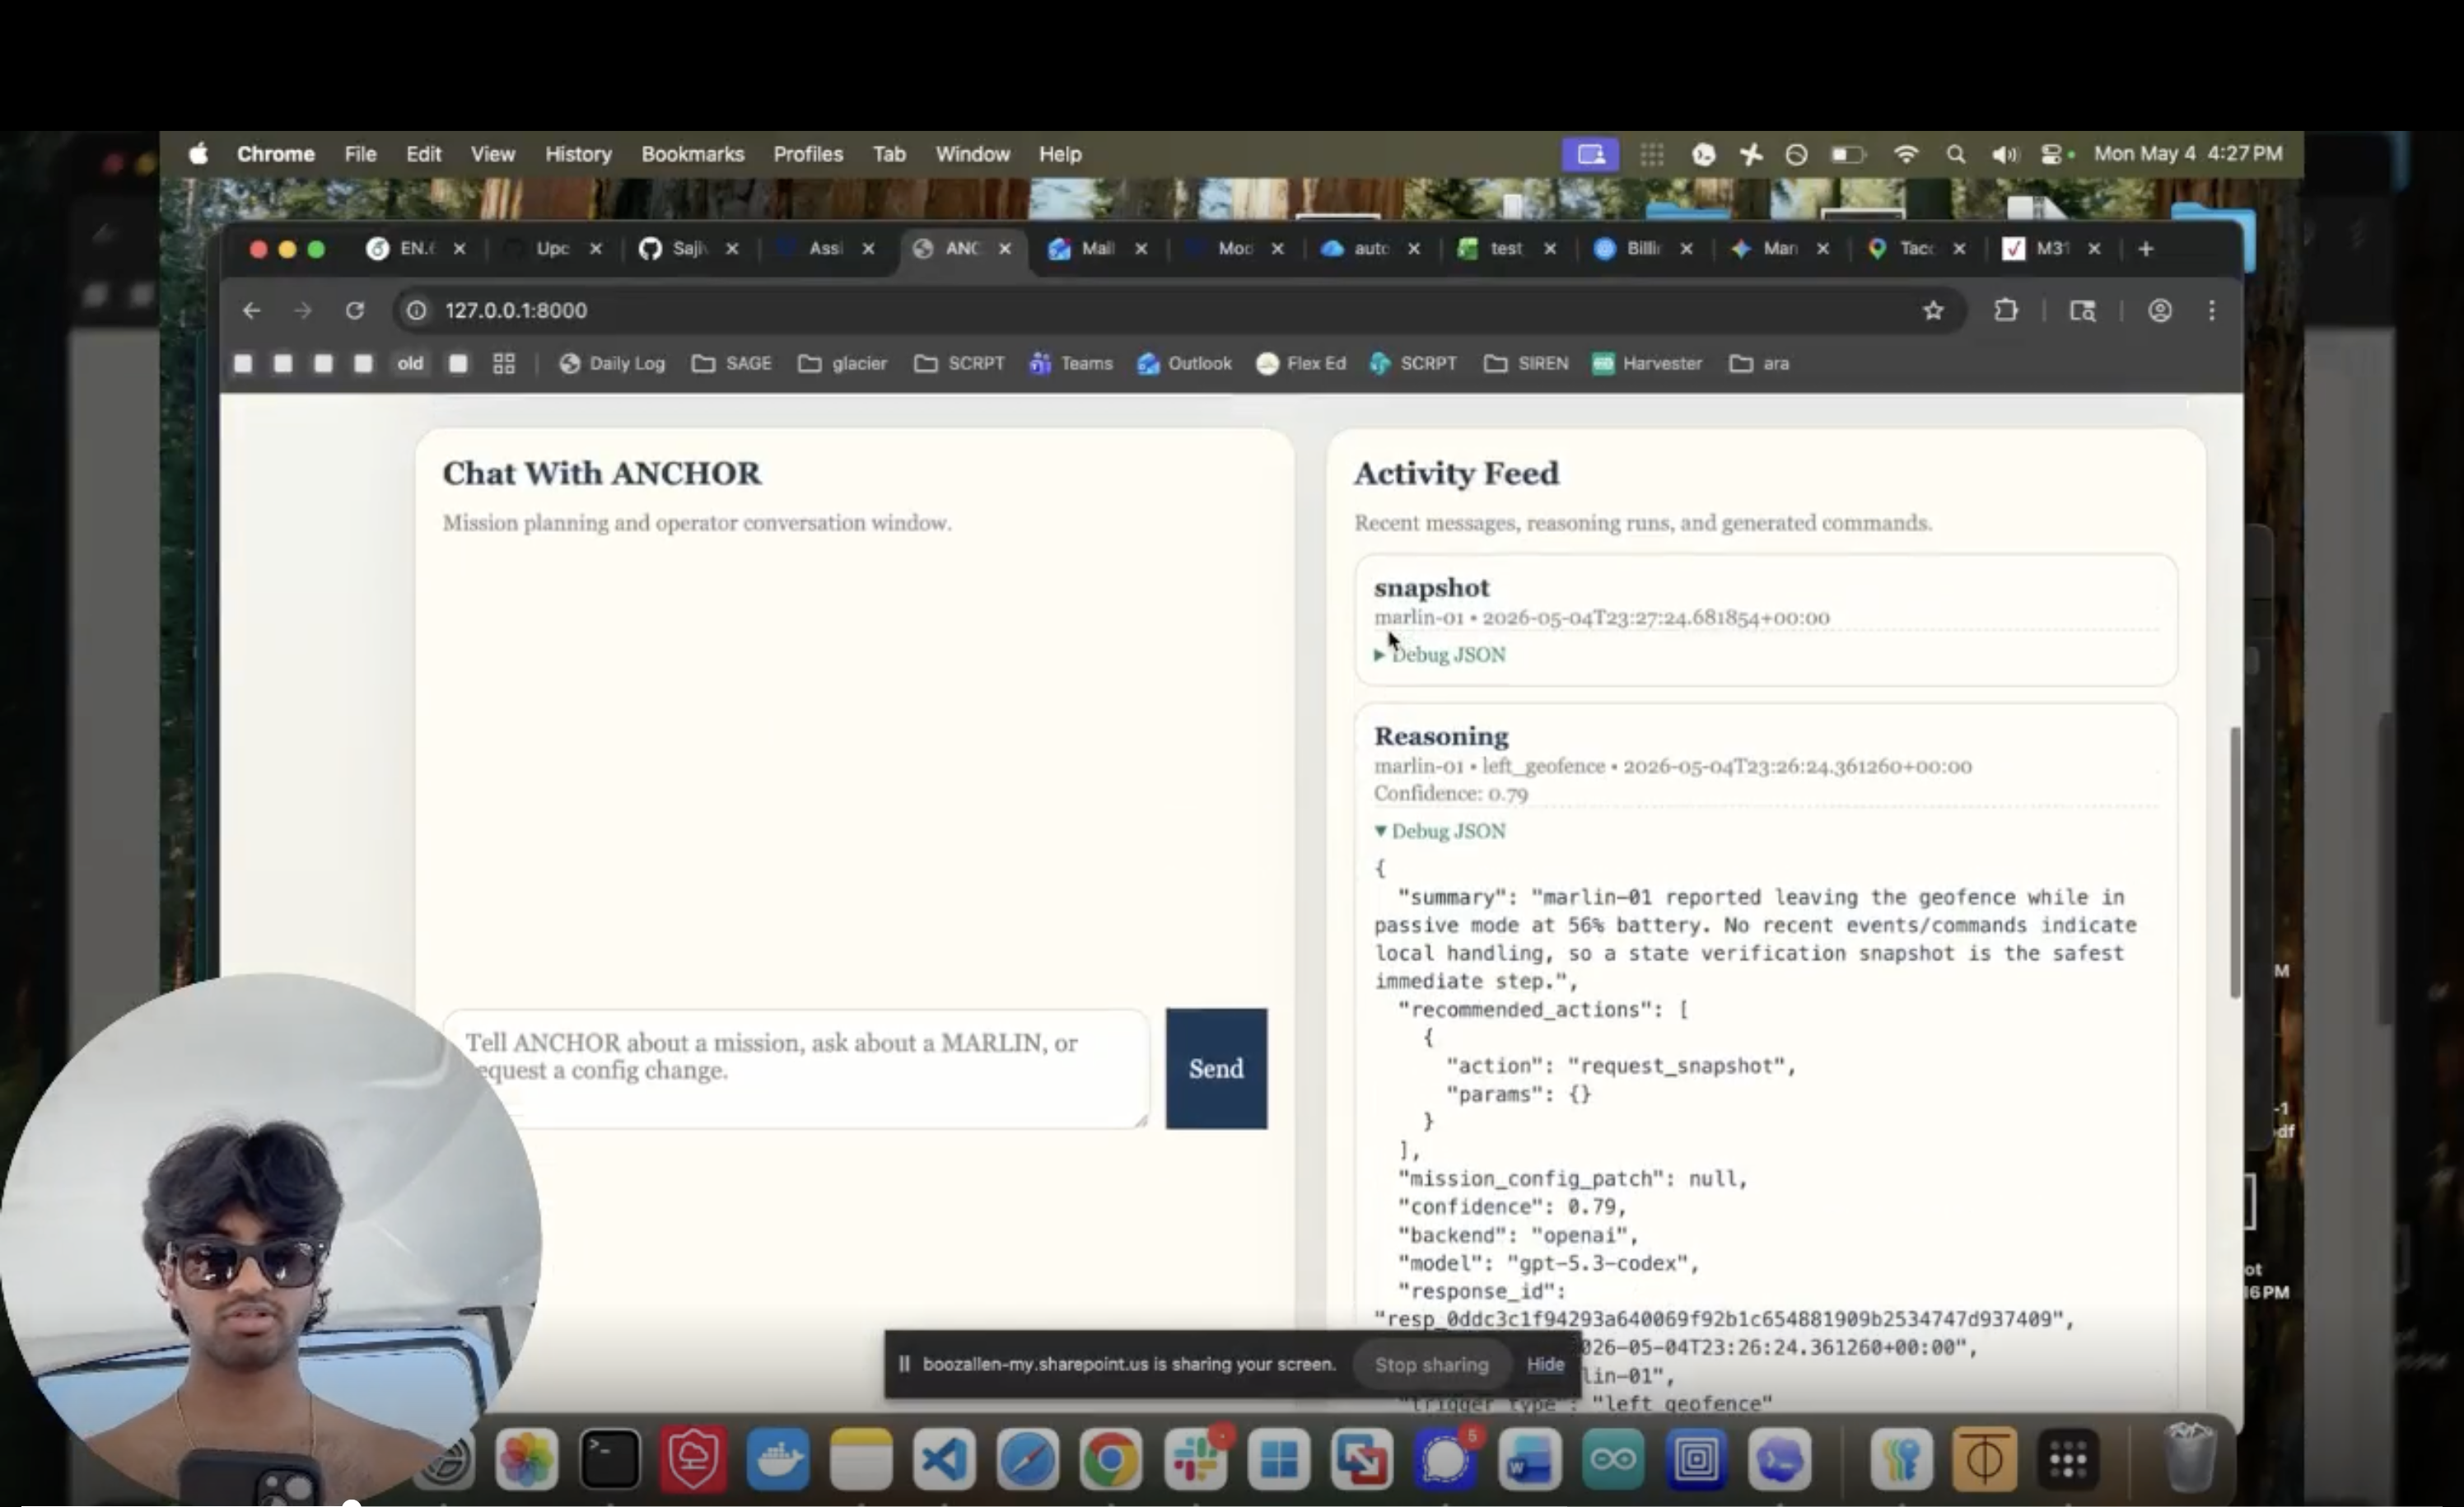
\includegraphics[width=\textwidth]{images/Codex Reasoning Anchor.png}
\end{minipage}
\caption{Dashboard evidence from the live field test. Left: ANCHOR showing MARLIN outside the configured geofence while the node remained in passive mode. Right: reasoning output generated during the run from live field telemetry and mission context.}
\label{fig:field-test-dashboard}
\end{center}
\end{figure*}

When the vessel entered the geofence, MARLIN's mission handler detected that its live coordinates were inside the configured boundary and autonomously transitioned the node into active mode. This transition triggered the reasoning engine, which invoked Codex and produced a Wi-Fi scanning recommendation based on geofence entry and the current battery condition. Wi-Fi scanning then began automatically, and nearby wireless networks were displayed in the ANCHOR interface. While the node remained inside the geofence, scanning continued as expected.

\begin{figure*}[t]
\begin{center}
\begin{minipage}{0.48\textwidth}
\centering
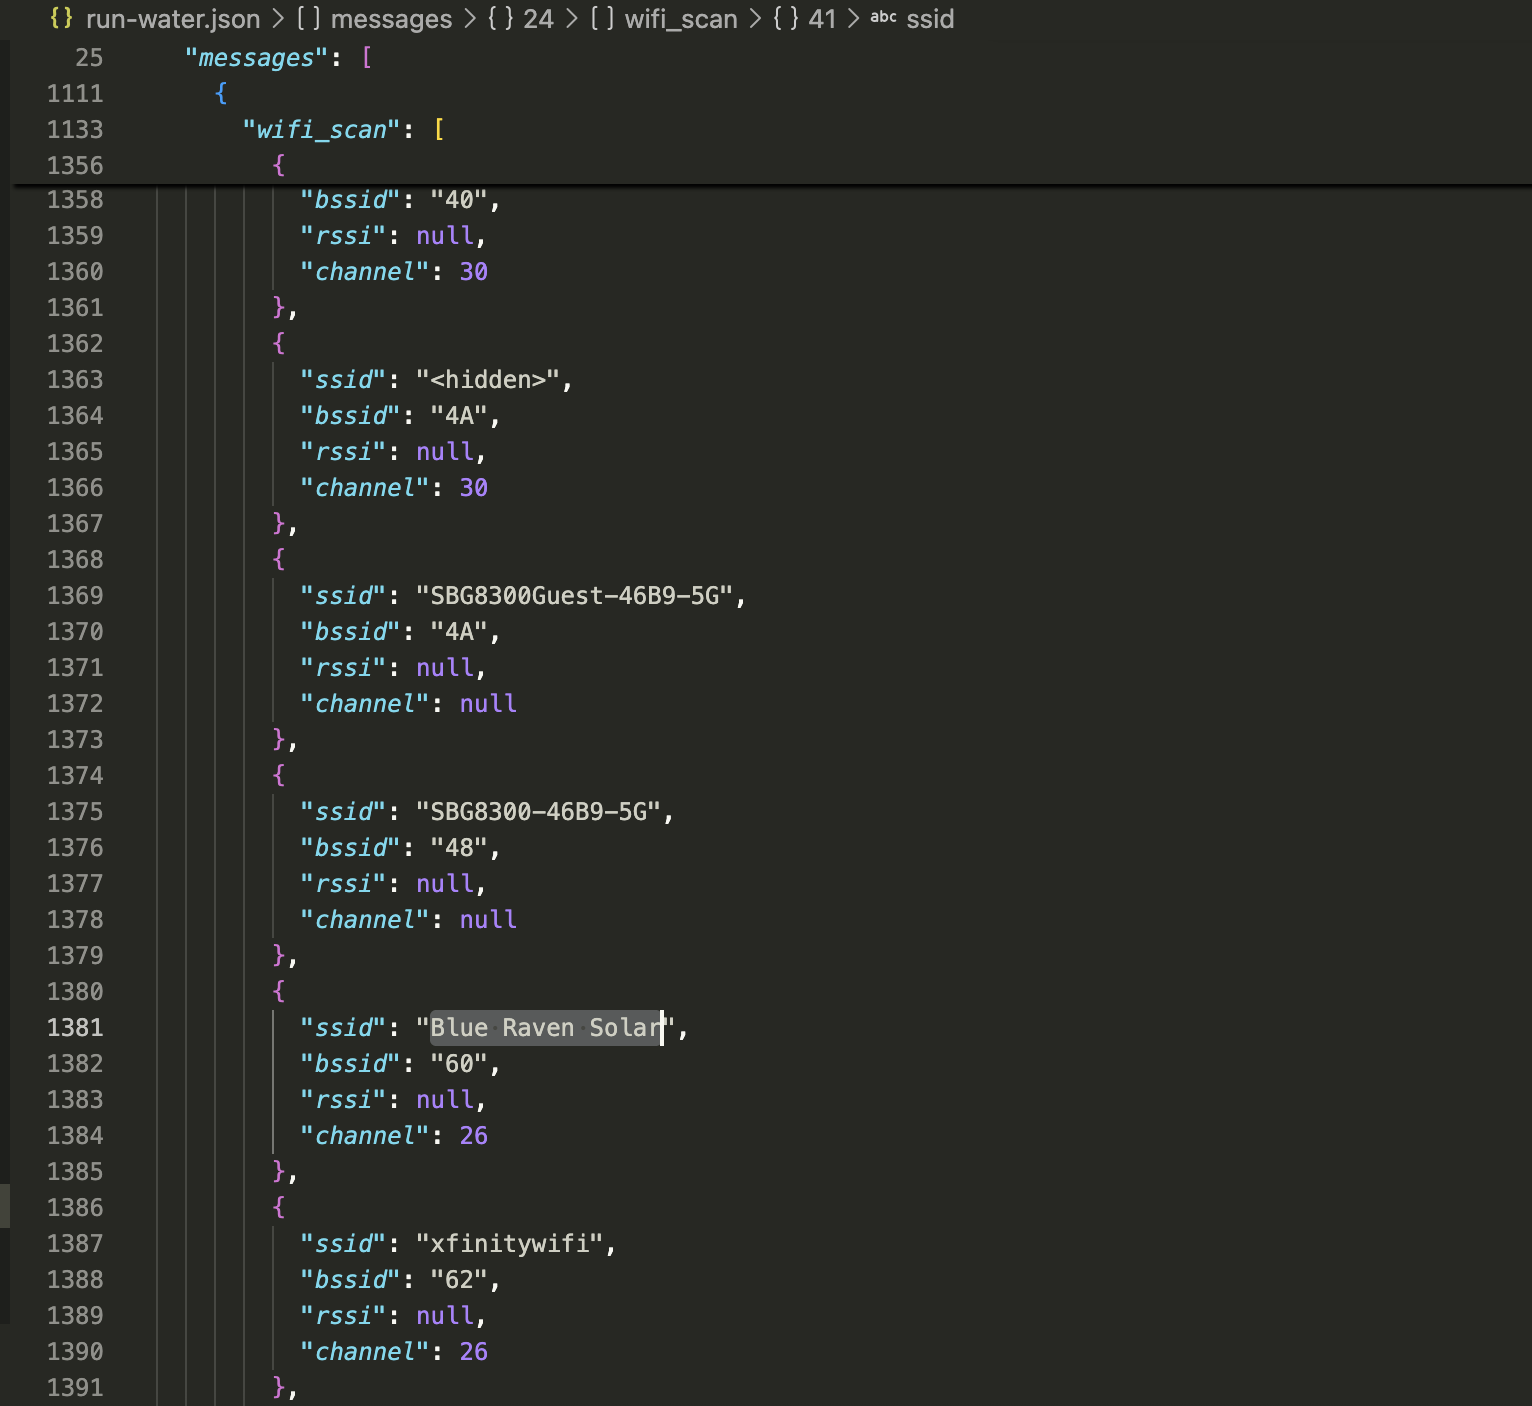
\includegraphics[width=\textwidth]{images/wifi found by marlin.png}
\end{minipage}\hfill
\begin{minipage}{0.28\textwidth}
\centering
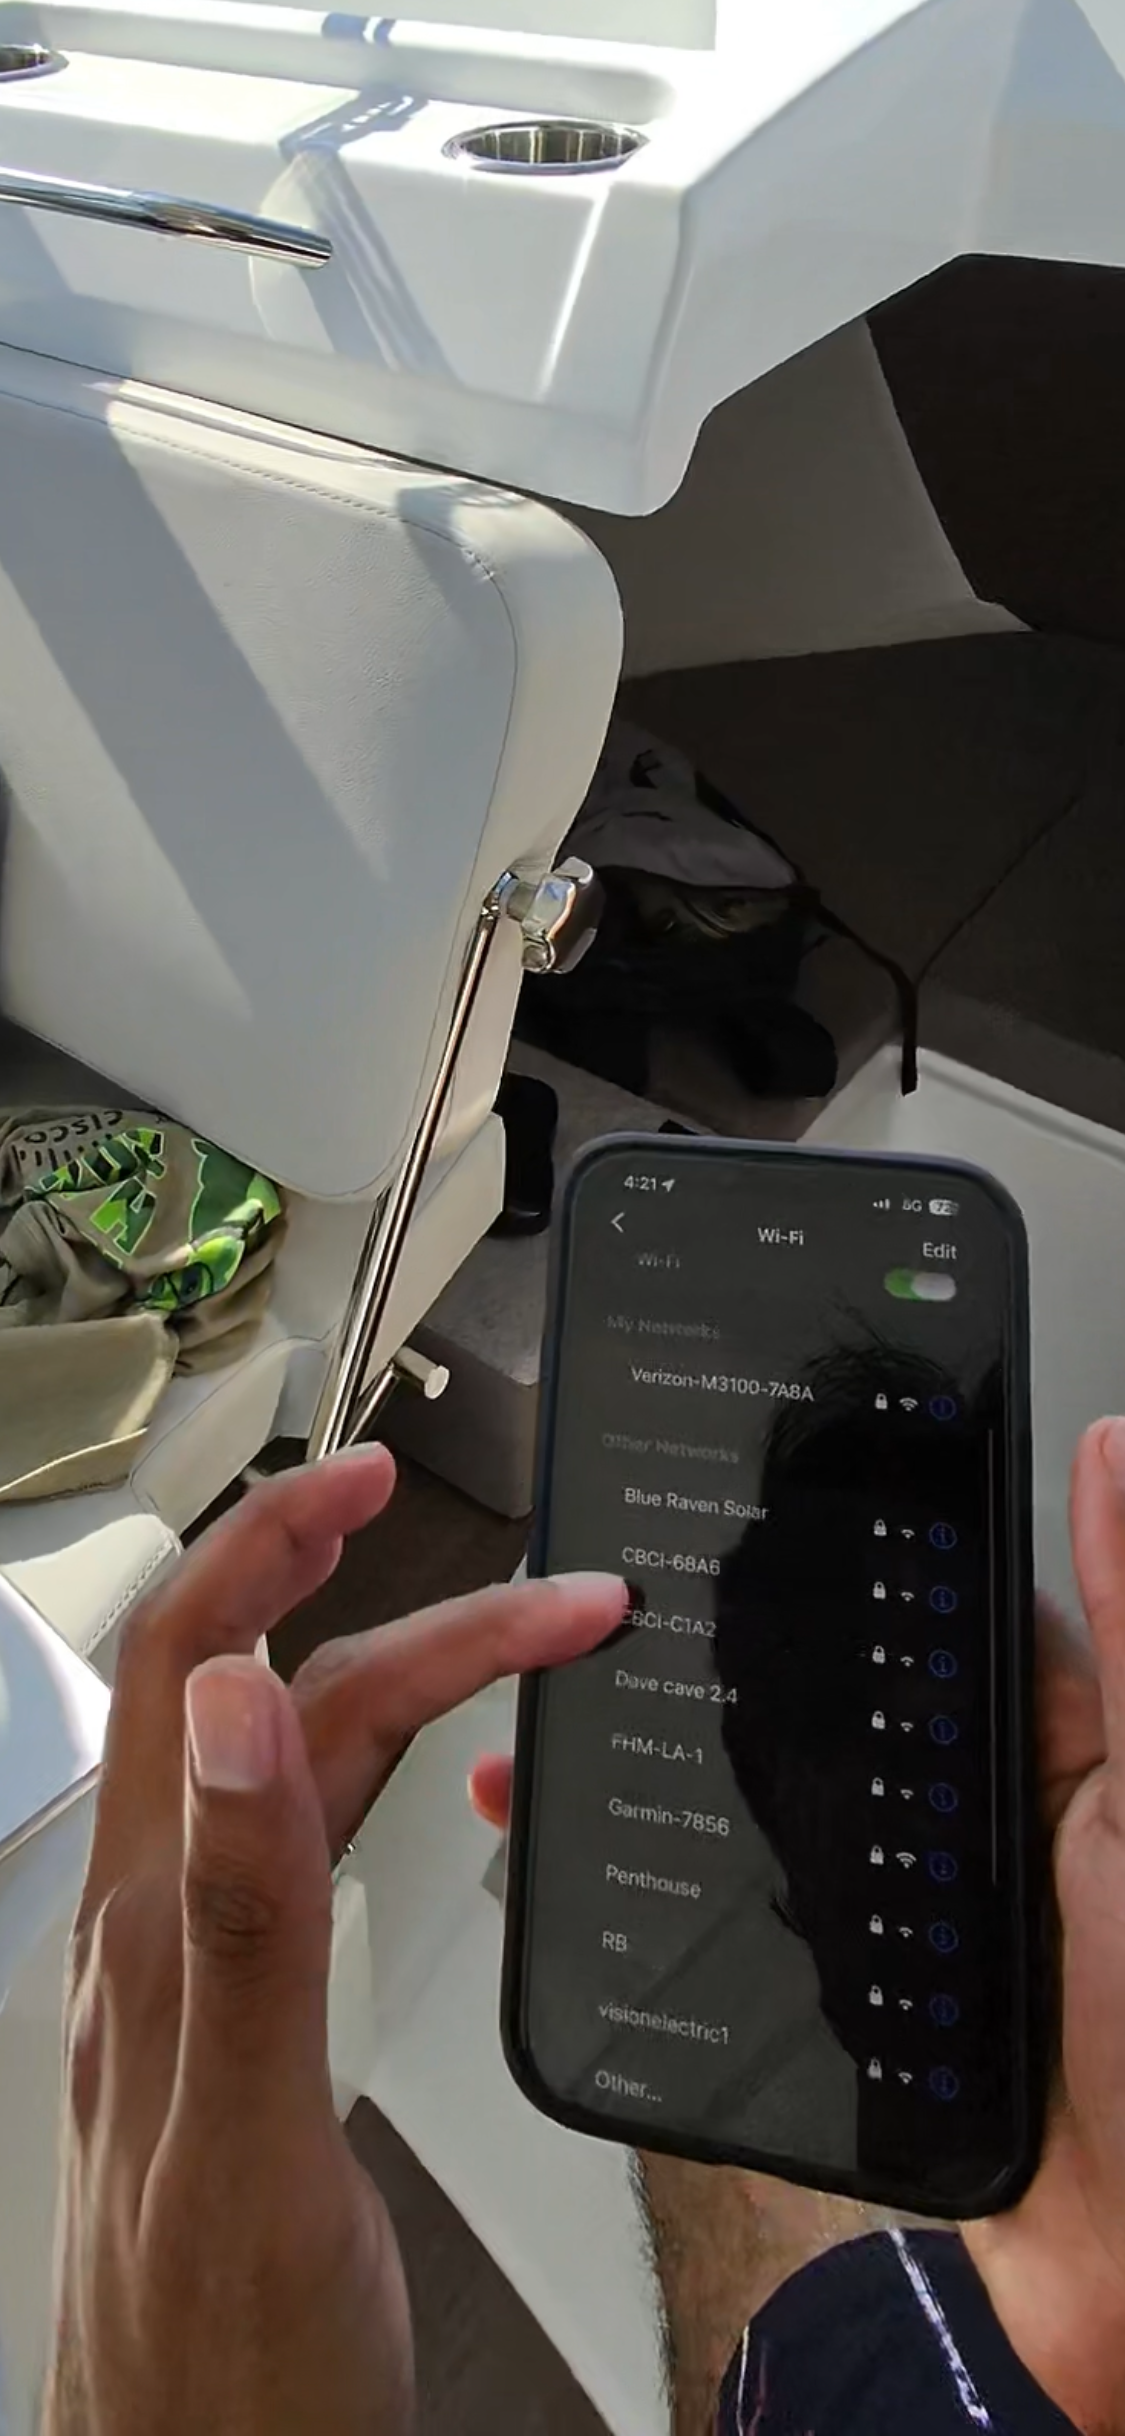
\includegraphics[width=\textwidth]{images/iphone blue wifi.PNG}
\end{minipage}
\caption{Wi-Fi evidence collected during the field test. Left: MARLIN-reported Wi-Fi scan output captured from the live run. Right: a phone-based view of nearby Wi-Fi networks in the same environment, including the Blue Raven Solar network referenced during testing.}
\label{fig:field-test-wifi}
\end{center}
\end{figure*}

After the vessel drifted through and exited the geofence, MARLIN returned to passive mode and scanning stopped. Later in the same run, when the Ubuntu laptop battery reached 20\%, MARLIN autonomously entered low-power mode. On a subsequent reentry into the geofence at approximately 6\% battery, MARLIN did not resume scanning. This behavior was consistent with the intended mission policy: low-power constraints should override discretionary sensing activity in order to preserve remaining energy. A manual attempt to force additional scanning behavior under that low-battery condition did not succeed.

This field run validated several core claims of the realized architecture. First, MARLIN successfully performed live GPS reporting to ANCHOR in a real maritime setting rather than only in simulation. Second, geofence-driven behavior changes occurred autonomously, with MARLIN locally handling mode transitions and ANCHOR providing higher-order reasoning and follow-up. Third, the node correctly suppressed scanning when battery state reached the low-power threshold, demonstrating that self-protective behavior could override mission-expensive activity even when the node reentered the mission area. Together, these observations provide real-world evidence that the hybrid ANCHOR/MARLIN system can autonomically enforce mission policy outside a purely simulated environment.

\begin{figure}[H]
\begin{center}
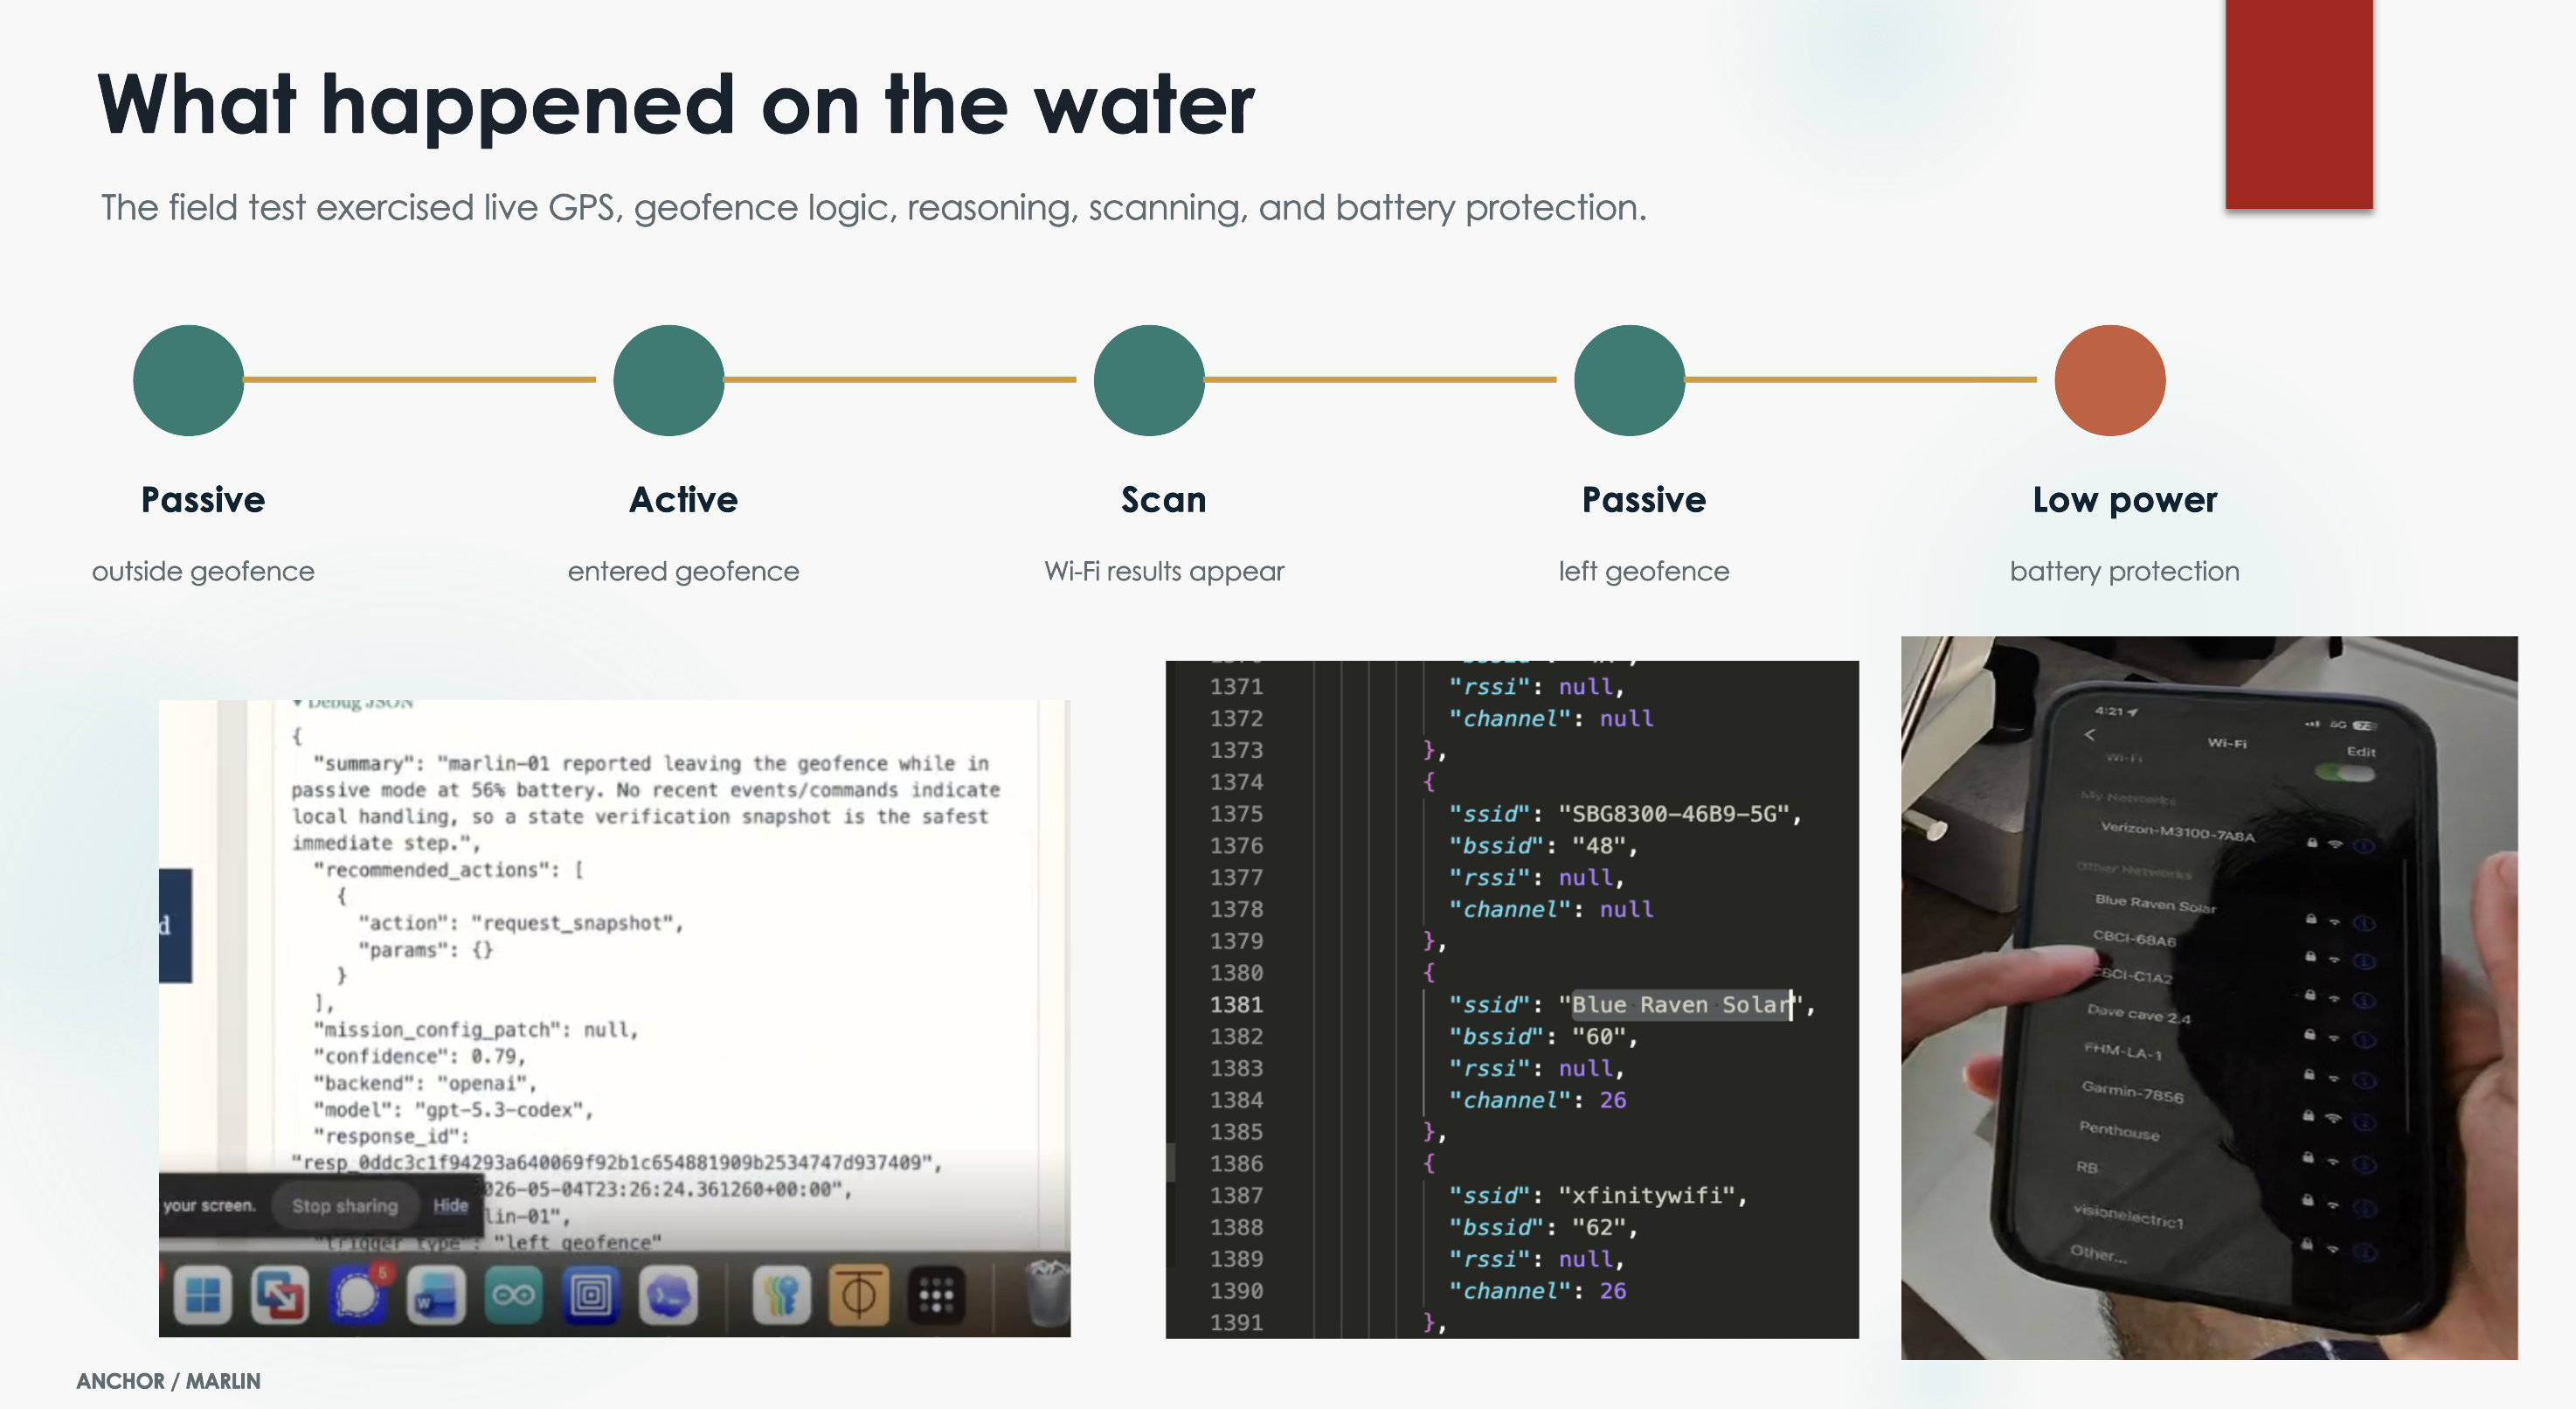
\includegraphics[width=0.48\textwidth]{images/harbor slide.png}
\caption{Overview of Harbor experiment, WiFi scans excerpt}
\label{fig:dashboard-scenario-runs}
\end{center}
\end{figure}

\subsection{Interpretation of Results}
These experiments show that the hybrid architecture is most successful when local policy enforcement and centrally assisted reasoning complement one another. Geofence transitions and low-battery behavior were handled particularly well because MARLIN could make immediate local state changes while ANCHOR provided mission-aware coordination. Target Wi-Fi detection also benefited from this structure, although the managed path in the current prototype primarily improved observability rather than producing a strong additional command sequence.

The weakest area of the system was command-failure handling. In both baseline and ANCHOR-managed modes, the operator still had to manually mark failure because the prototype did not reliably surface failed command responses back into the experiment harness. This limitation indicates that the realized architecture is stronger in mission-state autonomy than in execution-failure recovery.

\subsection{Data Collection and Metrics}
For each evaluation scenario, the system records telemetry, events, commands, command responses, and operator interventions. The goal of this data collection is not only to determine whether the system completed a scenario successfully, but also to measure how much operational burden was removed from the human operator.

The primary metric remains human intervention count. For each scenario, every instance in which a human operator must inspect telemetry, interpret node state, choose a response, or manually trigger an action is counted as an intervention event. The total number of intervention events required in the baseline system is then compared with the number required when ANCHOR is active.

In addition to the primary intervention metric, the following supporting measurements are collected:

\begin{itemize}
    \item \textbf{Scenario Completion Success:} Whether the node or fleet completed the intended behavior correctly.
    \item \textbf{Response Time:} The elapsed time between a triggering condition and the resulting response.
    \item \textbf{Command Outcome Counts:} The number of commands accepted, completed, rejected, or failed.
    \item \textbf{Mode Transition Counts:} The number of transitions between passive, active, and low-power modes.
    \item \textbf{Connectivity Recovery Behavior:} During communication-loss scenarios, the number of queued messages, duration of degraded operation, and success of later synchronization.
    \item \textbf{Reporting and Scan Behavior:} The frequency of telemetry and Wi-Fi scanning across passive, active, and low-power phases.
\end{itemize}

These metrics support both quantitative and qualitative analysis. Quantitatively, they are used to calculate intervention reduction and compare baseline performance to ANCHOR-managed performance. Qualitatively, they help explain how the realized hybrid architecture behaves under realistic mission conditions and where the main benefits and limitations of the current prototype emerge.

\subsection{Results Presentation}
The results are presented through summary tables, scenario-by-scenario comparisons, and visual evidence drawn from recorded telemetry and command history. The primary quantitative result is the comparison of intervention counts between the baseline system and the ANCHOR-managed system across all evaluation scenarios, which yields the overall percentage reduction in required human monitoring.

The included figures capture the main operational behaviors of the realized prototype:

\begin{itemize}
    \item A comparison of intervention counts by scenario and mode.
    \item Boat-based field-test images showing the physical deployment of ANCHOR and MARLIN.
    \item Dashboard screenshots showing geofence state, live telemetry, reasoning output, and Wi-Fi observations during the Tacoma run.
\end{itemize}

\section{Conclusion}~\label{conclusion}
The original vision of this project was a fully decentralized autonomic maritime node in which each MARLIN independently hosted a complete MAPE-K loop. The realized prototype demonstrates that many of those autonomic goals can still be preserved, but only through an architecture adapted to the practical realities of current LLM-based tooling, execution safety, and edge-device constraints. As a result, the project contributes both a working hybrid autonomic prototype and a concrete account of how ideal decentralized autonomy must be adjusted when implemented with present-day agentic systems.

The completed results strengthen that conclusion. In controlled scenario testing, the ANCHOR-managed configuration reduced operator interventions from five to one, corresponding to an 80\% reduction in human monitoring effort and exceeding the original 65\% target. In live field testing in Tacoma's Foss Harbor, the prototype successfully demonstrated real GPS reporting, autonomous geofence-triggered scanning, exit-triggered return to passive behavior, and low-battery suppression of mission-expensive sensing. At the same time, the experiments exposed a meaningful limitation: command-failure handling remains incomplete and still requires operator involvement. Beginning this project, I believed an LLM could fully run this system, and with the prototype of ANCHOR, I saw what could be successfully automated, and what limits still existed. I hope future research in this field continues to push autonomic computing to its fully realized state.

\bibliographystyle{IEEEtran}
\bibliography{references}
\end{document}
